% aa.dem % AA vers. 9.1, LaTeX class for Astronomy & Astrophysics % demonstration file % (c) EDP Sciences 
%-----------------------------------------------------------------------
%
%\documentclass[referee]{aa} % for a referee version
%\documentclass[onecolumn]{aa} % for a paper on 1 column
%\documentclass[longauth]{aa} % for the long lists of affiliations
%\documentclass[letter]{aa} % for the letters
%\documentclass[bibyear]{aa} % if the references are not structured % according to the author-year natbib style

%
\documentclass{aa}  

%
\usepackage{graphicx,svg,bm,amsmath,dsfont,siunitx,wasysym,tikz,color,scalerel}
%%%%%%%%%%%%%%%%%%%%%%%%%%%%%%%%%%%%%%%%
%\usepackage{comment}
\usepackage{hyperref}
%\usetikzlibrary{arrows,positioning,decorations.pathmorphing,backgrounds,calc,shadows}
%\tikzset{
%    ashadow/.style={opacity=.25, shadow xshift=0.1, shadow yshift=-0.1, color=red!50!black},
%    block/.style={rectangle, draw=black, left color=black!20, right color=green!60!, very thick, inner sep=1, outer sep=0, minimum width=25mm, text width=25mm, minimum height=20mm, text centered, drop shadow={ashadow}, rounded corners=2mm},
%    largeblock/.style={rectangle, draw=black, left color=black!20, right color=green!60!, very thick, inner sep=1, outer sep=0, minimum width=40mm, text width=40mm, minimum height=20mm, text centered, drop shadow={ashadow}, rounded corners=2mm},
%    largeblock2/.style={rectangle, draw=black, left color=black!20, right color=green!60!, very thick, inner sep=1, outer sep=0, minimum width=50mm, text width=50mm, minimum height=20mm, text centered, drop shadow={ashadow}, rounded corners=2mm},
%    textarea/.style={rectangle, draw=black, top color=cyan!30, bottom color=cyan, very thick, inner sep=1, outer sep=0, minimum width=25mm, text width=25mm, minimum height=15mm, text centered, drop shadow={ashadow}, rounded corners=1mm},
%    textarea2/.style={rectangle, draw=black, top color=cyan!30, bottom color=blue!50, very thick, inner sep=1, outer sep=0, minimum width=25mm, text width=25mm, minimum height=15mm, text centered, drop shadow={ashadow}, rounded corners=1mm},
%    textarea3/.style={rectangle, draw=black, top color=green!30, bottom color=cyan, very thick, inner sep=1, outer sep=0, minimum width=25mm, text width=25mm, minimum height=15mm, text centered, drop shadow={ashadow}, rounded corners=1mm},
%    largetextarea/.style={rectangle, draw=black, top color=blue!30, bottom color=magenta, very thick, inner sep=1, outer sep=0, minimum width=50mm, text width=50mm, minimum height=15mm, text centered, drop shadow={ashadow}, rounded corners=1mm},
%    largetextarea2/.style={rectangle, draw=black, top color=blue!30, bottom color=green!50, very thick, inner sep=1, outer sep=0, minimum width=50mm, text width=50mm, minimum height=15mm, text centered, drop shadow={ashadow}, rounded corners=1mm},
%    picframe/.style={rectangle, draw=black, thick, inner sep=0, outer sep=0},
%    dummy/.style={inner sep=0, outer sep=0, minimum width=0, minimum height=0},
%    myarrow/.style={->, >=latex', shorten >=1pt, very thick},
%    arrow/.style={=>, >=open triangle 90, very thick}
%}

%%%%%%%%%%%%%%%%%%%%%%%%%%%%%%%%%%%%%%%%
%\usepackage[options]{hyperref}
% To add links in your PDF file, use the package "hyperref"
\definecolor{midblue}{rgb}{0.0,0.4,0.7}
\definecolor{midgreen}{rgb}{0.0,0.8,0.3}
\definecolor{mypurple}{rgb}{0.8,0.2,0.8}
\newcommand{\edits}[1]{\textcolor{midblue}{#1}}
\newcommand{\fg}[1]{\textcolor{midblue}{#1}}
\newcommand{\fag}[1]{\textcolor{midpurple}{[FAG: #1]}} % with options according to your LaTeX or PDFLaTeX drivers.
%
\newcommand{\arrc}[1]{\begin{matrix}[c] #1 \end{matrix}}
\newcommand{\eqnl}[2]{\begin{eqnarray}\label{#1}#2\end{eqnarray}}
\newcommand{\floor}[1]{\left\lfloor #1 \right\rfloor}
\newcommand{\dd}[0]{\mathrm{d}}
\definecolor{midpurple}{rgb}{0.7,0.1,0.7}
\newcommand{\s}[2]{{#1}_{\mathrm{#2}}}


\begin{document} 

%MJK I would reform to "Forty years of Metsähovi radio observatory data of the Sun in the 37 GHz band"
%SKK There already is a paper of almost identical name
%MJK oh, but is this not then paper number II in that series? I mean, the title now binds us to presenting the radio butterfly diagram only. But I guess this is more or less the intent anyways.
  \title{Radio butterfly diagram from 40 years of Metsähovi solar observations
         on 37 GHz}
 
  \subtitle{I. Determining bias for Earth's atmosphere, solar limb brightening,
            and antenna beam convolution}
 
  \author{
    Sami Kivistö \inst{1,2}
    \and
    Merja Tornikoski \inst{1}\fnmsep
      \thanks{Contributions to antenna beam definition}
    \and
    Joni Tammi\inst{1}
    \and
    Juha Kallunki\inst{1}
    \and\\
    Maarit Käpylä\inst{2,3,4}
    \and
    Frederick Gent\inst{2,5}
  }

  \institute{
    Mets\"ahovi Radio Observatory (MRO), Aalto University,
      Mets\"aovintie 114, 02540 Kylm\"al\"a, Finland
    \and
    Department of Computer Science, 
    Aalto University, PO Box 15400, 00076, Finland
         \email{sami.k.kivisto@aalto.fi}
    \and
    Max Planck Institute for Solar System Research,
      Justus-von-Liebig-Weg 3, 37077 G\"ottingen, Germany
    \and 
    Nordic Institute for Theoretical Physics,
      Roslagstullsbacken 23, 106 91 Stockholm, Sweden 
    \and 
    School of Mathematics, Statistics and Physics,
      Newcastle University, NE1 7RU, UK 
  }
  \date{Received \today; accepted \today}

% \abstract{}{}{}{}{} 
% 5 {} token are mandatory
 
  \abstract
  % context heading (optional)
  % {} leave it empty if necessary  
  {
    Mets\"ahovi Radio Observatory has collected solar intensity maps for
    over $40$ years.
    Most data coverage is on $\SI{37}{GHz}$ frequency band.
    This data allows for analysis and identification of features over nearly
    four sunspot cycles, constituting roughly two solar magnetic cycles.
  }
  % aims heading (mandatory)
  %MJK Method paper: the aim should be to develop a method to extract some information from the data. Butterfly diagram is, as I understand, the only end product that we want to mention. That should perhaps be in the Results section of the abstract, right?
  {
    Analyze Metsähovi solar maps for years 1978 to present.
    Investigate for any features that would correlate with magnetic and
    sunspot activity.
  }
  % methods heading (mandatory)
  %MJK Method oriented paper: Detect HOW, Collapse HOW, Quantify HOW, Compare HOW
  %FAG The methods abstract needs to be compressed and most of this detail 
  %moved to the main text. Fred TODO
  %MJK Yes. It is good to bear in mind that the arXiv abstract field allows for 1920 chars... As we will submit there anyways, then it will be an additional pain, so better to conform to the char limits already now.
  {
    Determine the solar disk position and size from each map as well as
    normalize the measured background intensity for zero and the Quiet Sun
    Level (QSL) for unity.
    This can be done using a binary combination of two disk methods (1 and 
    2) and three normalization methods (a, b, and c).
    The methods are: (1) intentionally weighted center of mass of the radio
    sample coordinates, (2) fitting a circle for those sample coordinates
    which we, by geometry, expect to belong to the solar limb, (a) sort the
    intensity samples and detect the point of zero curvature from the index vs.     intensity dependency, the S-curve, (b) iteratively calculate the
    statistical mean and standard deviation of the intensity of 
    those points which are located within the solar disk and not too close
    to the limb, (c) detect two significant peaks from the intensity histogram,
    the lower intensity peak being the background and the higher the QSL.

    The method (2) can be augmented using two additional sets of information.
    When we observe exactly at the limb, we would expect $0.5$ QSL intensity
    due the the beam mixing disk and background signal.
    If one particular sample has intensity $0.4$ QSL, we would expect the
    sample to be slightly more away from the center.
    Collecting a large set of observations on different conditions, we can
    estimate how quickly the intensity drops as the beam passes the limb 
    from disk to background.
    Utilizing this limb profile, we can fine tune the position of each limb
    sample in the target set of (2) and proceed iteratively to obtain more
    accurate circle fitting.

    Any exceptional bright or dim features near the limb will affect the
    apparent shape of the solar disk in the map. 
    They will affect the outcome of the disk center position when we run the
    circle fitting algorithm.
    Bright features favour center fitting towards the feature,
    while dim features repel the center.
    We should thus exclude a sample from the target set of the circle fitting
    by proximity of any pre-determined bright or dim radio feature, since these
    features affect the apparent shape of the disk.
   
    Each radio sample is given heliographic coordinates as well as time of
    observation.
    We collect a two-dimensional histogram where each rectangular slot has a
    time range as well as a range of heliographic latitude.
    Integrating all the radio data, we aim to obtain a diagram analoguous to
    the famous butterfly diagram of sunspot activity.
    Assuming the diagram will have similar wing patterns as the sunspot
    butterfly, we will apply a feature detection for wing elements.
    We apply the same algorithm for the sunspot butterfly and compare the shape
    and duration of each wing.
  }
  % results heading (mandatory)
  {
    Radio butterfly diagram on $\SI{37}{GHz}$ frequency band.
    Identified solar cycles 21 to 24.
    Wing parameters from both the radio butterfly and the sunspot butterfly.
  }
  % conclusions heading (optional), leave it empty if necessary 
  %MJK This part sounds very good
  {
    We have developed a method for automatic feature detection from butterfly
    diagrams.
    This allows systematic comparisons between individual wings as well as
    different observational and simulated datasets showing butterfly a pattern.
  }

  \keywords{Solar physics, radioastronomy, butterfly diagram, solar cycle}

  \maketitle
%-------------------------------------------------------------------

\section{Introduction}

  %MJK References required. FAG: added, sufficient?
  The solar magnetic field is known to switch polarity in a full cycle of 
  approximately % ca. FAG abbr. -->  full word convention
  22 years, which consists of two sunspot cycles \citep{HEN19,Babcock61}.
  At %In FAG In --> AT
  the beginning of each sunspot cycle, the solar magnetic field is an axial
  dipole.
  %FAG reworded
  %Due to differential rotation, this field, being dominantly axisymmetric and running mainly in meridional planes, hence being dominantly 
  %poloidal, is transformed into an azimuthal field with the azimuthal direction being opposite between opposite hemispheres.
  %Solar differential rotation transforms the predominantly axisymmetric
  %Poloidal magnetic field into an azimuthal field with a 
  %MJK typo tendancy; but is it only a tendency? 
  %FAG: I interpreted tendency as approximate; reworded to avoid ambiguity
  %tendency
  %for opposite
  %polarity between hemispheres.
  Solar differential rotation transforms the predominantly axisymmetric
  poloidal magnetic field into an azimuthal field with opposite
  polarity between hemispheres.
  %MJK This is the controversial part of the solar dynamo process, and we need to think how to phrase things here.
  In the presence of convection and the Coriolis force due to solar rotation,
  %FAG consistent tense
  %this azimuthal field will be further distorted by the $\alpha$-effect.
  this azimuthal field is further distorted by the 
  %MJK Needs clarification in words before bluntly introducing alpha effect. Also references are needed here.
  %FAG: added in response to MJK
  action of turbulent vortical flows stretching, twisting and looping the field,
  known as the 
  $\alpha$-effect \citep{SKR66,KR80}.
  %After ca. $11$ years, this has resulted in dipolar field of opposite polarity, 
  %FAG ca. --> appr, and tense
  %After approximately 11 years this evolves into a dipolar field with
  %MJK whereto 'this' refer is unclear.
  %FAG: clarified
  After approximately 11 years the large scale magnetic field
  evolves into a dipolar field with
  polarity reversed from its original sign
  and the next sunspot cycle begins.
  %FAG remove paragraph break and reword
  The full 22 year cycle comprises two such sunspot cycles.
  
  %The full magnetic cycle is ca. $22$ years and consists of two sunspot cycles.

  %FAG insert paragraph break
  %Each sunspot cycle begins with 
  %an axial dipole, after which various activity on the visible surface of the Sun will first increase, 
  %then reach maximum and again decrease to a minimum, while it migrates from high latitudes towards the equator. This is 
  %FAG reword the Sun --> Sun NASA capitalization convention
  %Each sunspot cycle emerges from the quiet Sun of an axial dipole as
  %MJK 'emerges from the quiet Sun of an axial dipole' sounds a bit odd.FAG: rephrased 
  Starting from a quiet Sun containing a relatively weak axial dipole 
  each sunspot cycle emerges as
  activity on the visible surface of Sun, typically near mid-latitudes
  %FAG Moved from below
  ($\pm20^{\circ}$ to $\pm 30^{\circ}$).
  While the frequency and coverage of the sunspots increases towards a maximum
  the location of the activity drifts equatorward. 
  This migration continues after the maximum with decreasing activity
  closer to the equator bringing the sunspot cycle to an end.
  This was first recorded in the Maunder butterfly diagram by Edward Maunder
  in 1904.
  %FAG: moved from below
  Since sunspots are a feature of Sun's magnetic field and as the solar
  magnetic field is mostly axisymmetric, 
  %MJK References needed here FAG: OK?
  the longitudinal location of the
  activity can reasonably be neglected \citep{PBKT06}.
  Considering this two-dimensional time-latitude histogram of sunspot activity
  or magnetic field intensity, similar butterfly 
  diagrams are also recovered from solar magnetograms
  %MJK Streamline the referencing here.
  %\citep{GHHZ83,VLMCS12}
  %and \citep[][and references therein]{LUSDADM17}.
  \citep{GHHZ83,VLMCS12,LUSDADM17}.
All our HPCE3 visitors from the spring period were paused an
  It is also reported for radio brightenings of the 17 and $\SI{34}{GHz}$ band
  \citep{Shibasaki13,SCGVPS14} and of $\SI{37}{GHz}$ \citep{metsahovi40}.
  \fag{add additional references in radio and visible data into above paragraph}
 
 
  %FAG comment below duplication
  %%MJK I think the toroidal field is evolving all the time; maybe better is to say during the dominance of the toroidal field?
  %
  %During the time of evolving azimuthal field, we observe various types of activity, such as sunspots, magnetic regions as well as radio brightenings. These features appear first in the middle latitudes ($\pm 
  %20^{\circ}$ to $\pm 30^{\circ}$) on both hemispheres. 
  %
  %%MJK Now the impression is that the distribution is bimodal; only at high and then only at low. Maybe to add 'progressively closer'
  %
  %Later in the cycle, they appear closer to the equator. 
  %%MJK I would say something on the lines: '
  %
  %%FAG moving this into the previous paragraph above
  %As the solar magnetic field is mainly axisymmetric, a longitudinal average is suitable. Taking such an average, resulting in a two-dimensional time-latitude histogram, reveals the preferred locations of magnetic activity on patterns that resemble butterfly wings...
  %The 
  %density of a preferred activity will be integrated into a two-dimensional histogram, which show the average density as a 
  %function of time and heliographic latitude. This is known as a butterfly diagram, and was first constructed for 
  %%MJK Kallunki papers are most likely not sufficient reference for the magnetic butterfly diagrams, only for radio brightenings. 
  %sunspots and later for magnetic regions and radio brightenings \cite{metsahovi40}.
 
  %FAG adding addition context
  From sunspots and magnetograms of the photosphere we have relatively rich
  %MJK hyphen ?
  %well resolved 
  well--resolved
  data about the 
  %MJK should perhaps be written out, when used for the first time, same for 3D.
  %FAG: OK done
  two-dimensional (2D) 
  evolution of the solar surface magnetic 
  field, but observation of the three-dimensional (3D)
  structure of the field is limited by the 
  weakness of magnetic measurements from the solar atmosphere relative to the
  surface.
  %FAG reworded and expanded 
  Mets\"ahovi radio observatory (MRO)\footnote{
  \href{https://www.aalto.fi/en/metsahovi-radio-observatory}{
        https://www.aalto.fi/en/metsahovi-radio-observatory}}
  is observing emissions, primarily in
  $\SI{37}{GHz}$ frequency band, dating back over forty years.
  This is in the frequency range suitable for detecting non-thermal emissions
  from high energy electrons associated with active-region magnetic fields, so
  is a good proxy for the intensity of the magnetic field.
  These are also well suited to observing the thermal emissions from the quiet
  Sun.
  Comparing and contrasting the maps from these emissions with other
  observations can help to reveal more about the structure of the magnetic
  field in plasma of varying temperature and by inference height.
  Furthermore, the data incorporates almost four magnetic cycles, yielding
  a valuable resource to investigate long-term variation within and bewteen 
  cycles, alongside and in contrast to other sources.
  %Metsähovi radio observatory (MRO) has collected solar maps since 1978. Most of these maps are recorded on 
  %%MJK Fred is better with the language, but I make the following notions:
  %%MJK 'in 37 GHz frequency band', 'a valuable', 'long-term'
  %$\SI{37}{GHz}$, which is valuable resource for analyzing long term solar evolution.
  %%MJK What kind of solar activity does 37GHz trace? This is an important point to clarify.
  %FAG added new para break

  \fag{add paragraph reviewing previous Mets\"ahovi publications and references}
  %MJK One should explain in more detail what Kallunki has already published from this data.

  %FAG I have summarised the rest of the introduction to keep it concise and
  % have copied the rest to the methods section, where it is better suited.
  Across the lifetime of the MRO the equipment has experienced several upgrades
  and evolution of the data format.
  This article shall describe the pipeline of data processing to transform the
  raw data into a time series of solar radio maps, normalised, corrected for
  instrumental bias, atmospheric noise and effects, time of day and seasonal
  effects and solar 
  %MJK lim typo
  limb dimming effects.
  We present two methods for correctly detecting the position of the solar disk
  in each map and three methods for normalizing the signal levels, such that
  the background \emph{black sky} 
  %MJK is 
  has value zero and the 
  Quiet Sun Level (QSL) value unity.
  The maps are then projected from RA and Dec onto their rotating heliographic
  surface coordinates.
  We also introduce tools we have prepared for automatic tracking of active 
  regions, which are suitable for any magnetograms or similar maps, and which
  we shall apply in detail in future publication.
  This is 
  %decribed 
  described in Section\,\ref{sect:methods}.

  %MJK 'From this' does not sound understandable. 
  From this we present a time-latitude histogram of the radio intensity,
  including previously inaccessible machine-drawn maps from 1978 -- 1987 and
  up to 2020.
  This yields the most complete time series thus far available from MRO, 
  spanning almost completely the last four sunspot cycles.
  We compare our butterfly diagram with one constructed from the sunspot 
  counts during the same epoch.
  The are presented in Section\,\ref{sect:results} together with some 
  examples of our active region tracking.
  Finally, we discuss in Section\,\ref{sect:discussion} 
  %MJK some 
  how the radio 
  observations differ from other solar observations, 
  %MJK Consistency with Shibasaki could be left to be said later.
  consistent with the 
  results of \citet{Shibasaki13}. 

  %FAG the residual text has been copied to Methods 
  %During the 40 years, the equipment 
  %has experienced several upgrades and there has also been changes in the data format.
  %he data requires careful 
  %normalization procedures, after which the butterfly diagram can be constructed from the solar maps. The solar maps from 
  %1978 to 1987 were originally recorded on magnetic tapes, out of which the data was rendered on contour maps using a 
  %mechanical plotter. Since then, the magnetic tapes have been lost, and the maps were only available as 
  %%MJK it would not hurt to stress that they were printer on paper only -> plots -> printouts.
  %these plots.
  %%MJK or rather pattern recognition?
  %Using various image recognition techniques featured in \cite{masterthesis}, these contour maps were converted back into 
  %numerical form. For these prepared contour maps, 
  %%MJK Define better what you mean by 'solar disk being available'. It might not be clear to a common reader.
  %the solar disk was already available, while for the later maps from 
  %1989 to present the disk 
  %has to be detected using automatic image recognition. 
  %%MJK To make it more clear:
  %%MJK The purpose of this paper is to present two methods () for detecting the disk and ....
  %We present two methods (1: S-curve and 
  %center of mass, 2: convex hull) for detecting the disk and three methods (a: S-curve and constant fraction, b: 
  %statistics and outlier neglection, c: interpolating between histogram peaks) for normalizing the signal levels so that 
  %zero is the black sky at the background and unity is the Quiet Sun Level (QSL).
  %%MJK Then there should be a sentence stating that "As our final data product we present here a butterfly diagram of radio brightenings extending over the full time span of the recorded Mets\"ahovi solar data set".
  %
  %%MJK This would be better in the methods section, to outline the general workflow from the raw data to the final product.
  %When the disk fitting is done, every radio sample can be projected into rotating heliographic surface. We use the 
  %Carrington coordinates for this. As every sample now has time, heliographic latitude, and intensity relative to QSL, we 
  %can average them on a two-dimensional grid in order to obtain a butterfly diagram. The sunspot data is already in a 
  %format that has latitude and time bins, so simple interpolation is needed to convert it into the same domain as our 
  %butterfly. For radio data, the measurable quantity is the intensity, while for the sunspot data it is the fraction of 
  %area covered by sunspot, between two arcs of constant latitude.
  %
  %Having obtained the butterfly 
  %%MJK diagram?
  %diagrams, we 
  %%MJK We should imply that more analysis is to come later.
  %%MJK "We also perform a preliminary analysis of the obtained butterfly diagram, by performing feature detection algorithm ... that is discussed in section BLAA. Our preliminary findings are presented in Section BLAA2."
  %perform feature detection in order to get quantified information on the wing 
  %shapes. 
  %%MJK Again, introduction might not be the best place to describe the workflow, but the methods section.
  %This is done iteratively, starting with the each hemisphere and predefined solar cycle start and end times 
  %(later: wing). For each wing, we give the high intensity cells a considerable weight and fit a polynomial of a desired 
  %degree to the time-latitude domain. This gives the wing shape and root. Statistical variance with respect to the root 
  %gives us the wing thickness, which can be assumed a constant or a polynomial function of desired degree. We fit the 
  %third polynomial in the time,intensity domain, where the intensity is averaged over the wing latitudes for each time 
  %cell. The relevant roots or local minima of this intensity polynomial give the begin and end times for each wing. Having 
  %now quantified the shape and dimensions of each wing, we can neglect any outlier cells from the grid and perform several 
  %iteration steps to refine the shape. In the last stage, all the wings will coexist in the same grid, which now contains 
  %all the 40 years of data from both hemispheres. We will set the weights to zero for those cells which would have 
  %overlapping wings, in order to encourage the algorithm to produce non-overlapping wings. We tried several sets of 
  %parameters, while the most promising fits were produced with first order wing shape and thickness and fourth order 
  %intensity profile.
  %
  %%MJK So, to summarize my comments to the intro: expand significantly on Kallunki earlier paper(s), and pinpoint in detail what was there, and what is new in here, and why this work was necessary. Expand on the relevance of the dataset: what does 37GHz data describe, why is it relevant, what else has been done before in the frequency band? Move the parts describing the workflow to Section 2.
  %
%--------------------------------------------------------------------

  \begin{figure}
  \centering
  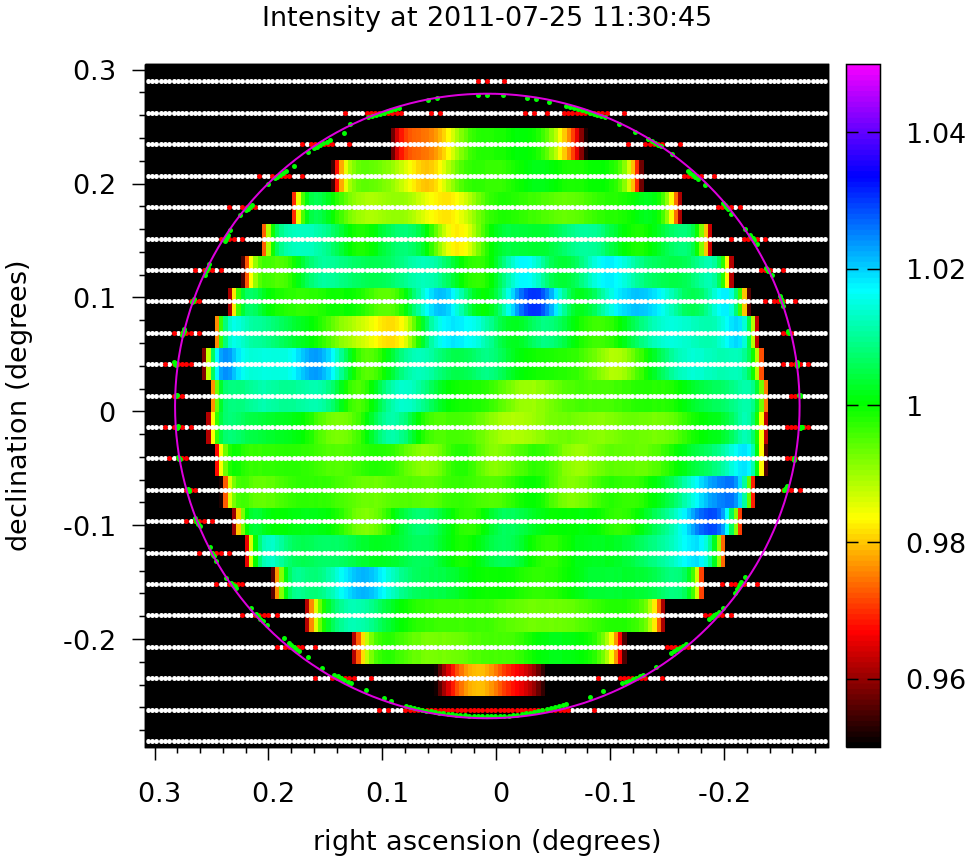
\includegraphics[trim=0cm 3cm 0cm 1.2cm,clip=True,width=\columnwidth]{nea1311582408.png}
  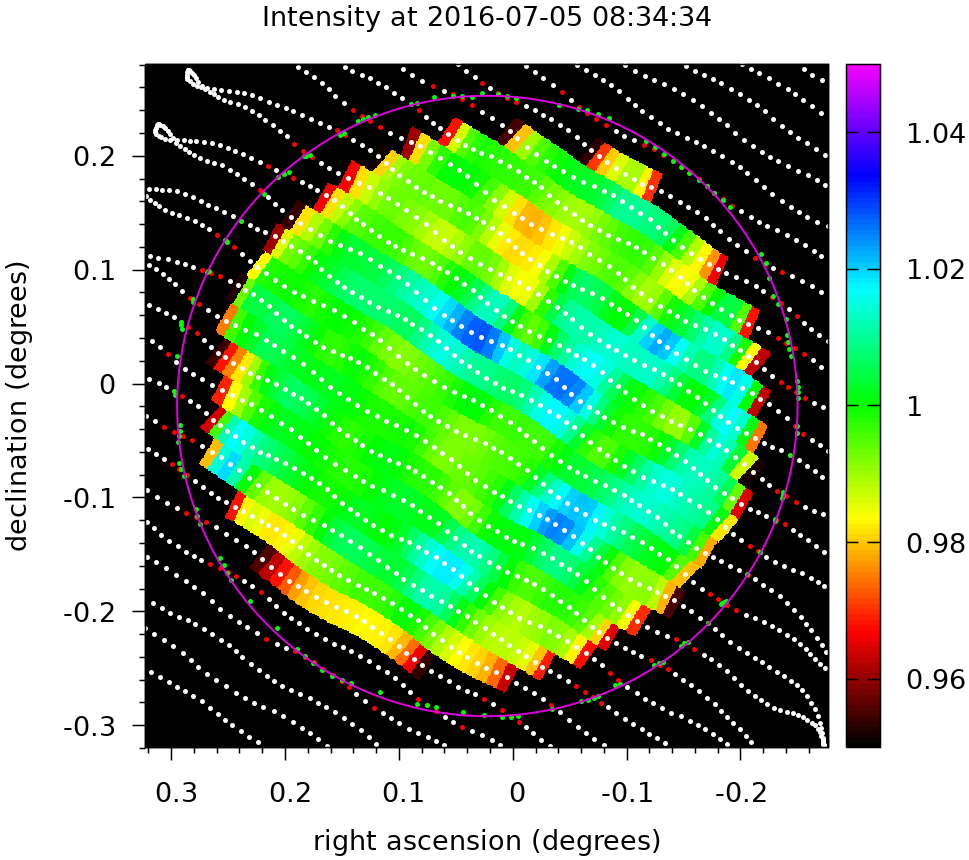
\includegraphics[trim=0cm 0cm 0cm 1.2cm,clip=True,width=\columnwidth]{nea1467696874.png}
  \caption{
    Typical Mets\"ahovi solar observations on $\SI{37}{GHz}$ {\bf(a)}
    25.07.2011 and {\bf(b)} 05.07.2016.
    Prior to May 2015 the observation beam scans along the equator, with
    samples mapped onto a rectangular grid.
    Since June 2015 a more accurate fit to the beam path was used, scanning 
    horizontally.
    %Maps that originate May on 2015 or earlier have
    %sweeps along the equator. Samples are assumed on a rectan-
    %gular grid. Typical Metsähovi solar observation on 37 GHz.
    %This data format has been in use since June 2015. White
    %dots: samples not used for disk fitting. Red dots: sam-
    %ples used for disk fitting, radial offset calculated based on
    %limb model. Green dots: samples corrected for radial offset,
    %which constitute the target set for circle fitting. Color map:
    %each pixel is mapped to the nearest observational sample.
    %Comment: This is an original uncalibrated map. Explain
    %what is added up as part of calibration. Include another
    %plot with the final version in Solar coordinates.
  \label{oldmap}\label{typicalmap}}
  \end{figure}
\section{Methods}\label{sect:methods}

\subsection{Data sources}\label{sect:source}

  During a typical measurement, the antenna beam makes a sweep across the
  visible solar disk (Figure \ref{typicalmap}).
  The data comprises three sources:
  \begin{enumerate}[A]
    \item
    The solar maps from 1978 to 1987 were originally recorded on magnetic
    tapes, from which the data was rendered onto paper contour maps using a
    mechanical plotter.
    Subsequently the magnetic tapes were lost, so that only the printed maps
    were 
    %MJK one too many 'only's
    %only 
    available. 
    Applying pattern recognition techniques developed by
    \cite{masterthesis}, the scans of the paper contour maps were converted
    back into a numerical form, consistent with that of 
    %MJK This might not be understandable stand alone. One could add smthg like "the digital format currently used for reconrding new maps".
    the later digital format.
    The solar disk position was already marked on these paper maps.
    \item
    Until the end of May 2015 the maps were scanned in the equatorial direction,
    so that declination is shifted between adjacent sweeps, as displayed in
    Figure\,\ref{typicalmap}{\bf(a)}.
    The maps assume linear antenna tracks with constant speed and sample rate.
    \item
    After June 2015 the sweeps have been horizontal, with shifting altitude
    between sweeps, as shown in Figure\,\ref{typicalmap}{\bf(b)}.
    These modern maps respect the true path of the antenna, typically recorded
    with $25$ samples per second for two minutes.
    %MJK The final map in solar coordinates is presented in Figure 1(c)...
  \end{enumerate}

  The digital maps do not include the location of the solar disk.
  The disk markings in Figure\,\ref{typicalmap}, are identified by the 
  disk fitting method(s), described in Section\,\ref{sect:disk}.
  The intensity ranges shown in Figure\,\ref{typicalmap} are the original
  uncalibrated levels.
  For these, as well as those recovered from the earlier paper prints, the 
  signal levels need to be normalised, to correctly identify the 
  %MJK Quiet Sun level? Has this been introduced earlier?
  %MJK It was introduced later, now swapped.
  quiet Sun level (hereafter QSL) and the
  black sky, also explained in Section\,\ref{sect:disk}.

  %
  %%MJK I think it would be best to put figures 1 and 2 into one single figure, and maybe add there also the planned figure of the final map in solar coordinates (Fig 1 caption). Also, the older map should become before the more recent map. 
  %During a typical measurement, the antenna beam makes a sweep across the visible solar disk (Figure \ref{typicalmap}). 
  %Until the end of May on 2015, the maps have been scanned in equatorial direction, so that declination is shifted between
  %%MJK This would become Figure 1(a).
  %adjacent sweeps. Since June, 2015, the sweeps have been horizontal, with shifting altitude between sweeps. 
  %%MJK This would become Figure 1(b).
  %These modern 
  %maps respect the true path of the antenna, while the older maps have assumed linear antenna tracks with constant speed 
  %%MJK typo
  %and 
  %%samplerate 
  %sample rate along the equator as in Figure
  %%MJK Figure 1(b).
  %\ref{oldmap}. The new maps typically recorded with $25$ samples per second for two minutes.
  %%MJK The final map in solar coordinates is presented in Figure 1(c)...
  %%MJK Horizontal row/vertical column of panels, up to Sami to decide...


\subsection{Heliographic coordinates from radio data}

A particular radio data sample $s_i$ contains time $t_i$, relative position on the sky $(\delta \mathrm{RA}_i, \delta 
\mathrm{dec}_i$), and measured intensity $u_i$ in arbitrary linear units. For convenience, we use two equivalent 
conventions for sample notation:

%MJK Introducing line break to fit the equations on a single line
%\eqnl{radio_sample}{
%s_i = \left( t_i, \delta \mathrm{RA}_i, \delta \mathrm{dec}_i, u_i \right) = \left( t(s_i), \delta \mathrm{RA}(s_i), \delta \mathrm{dec}(s_i), u(s_i) \right) \text{.}
%}
\eqnl{radio_sample}{
s_i &=& 
\left( t_i, \delta \mathrm{RA}_i, \delta \mathrm{dec}_i, u_i \right) \\ \nonumber
&=& \left( t(s_i), \delta \mathrm{RA}(s_i), \delta \mathrm{dec}(s_i), u(s_i) \right) \text{.}
}
%Observation is done at time $t_i$ and from geographic location 
%$(\phi_{\earth}, \lambda_{\earth}) = \left( +60.217797339^{\circ}, +24.393084663 \right)$, which is 
%Metsähovi Radio Observatory.
Each scan $S = \left\{ s_i \right\}_{i=\s{i}{min}}^{\s{i}{max}}$ consists of maps taken 
during $\s{t}{min}(S) \le s_i \le \s{t}{max}(S), \; s_i \in S$.
The equatorial coordinates used are relative to the expected position of the central point
of the Sun at $t_i$ and they are cosine corrected to have unit aspect ratio:
\eqnl{relative_radec}{
\delta \mathrm{RA}_i  &=& \frac{\mathrm{RA}_i - \mathrm{RA}^{\astrosun}(t_i)}{\cos \left( \mathrm{dec}^{\astrosun}(t_i) \right)} \\
\delta \mathrm{dec}_i &=& \mathrm{dec}_i - \mathrm{dec}^{\astrosun}(t_i) \text{.}
}
%In this work, we study only samples taken on $\SI{37}{GHz}$.
%The raw intensity $u_i$ is measured in arbitrary units.
Our solar maps are not sensitive to small systematic pointing errors or inter map variations in signal levels, since we calibrate each scan individually.
% determine the position and size of the solar disk as well as signal levels in the background and within the quiet sun area.
%MJK not to confuse the reader, refer already forward
We apply algorithm $F_j$,
%MJK
defined in detail in Sect.~\ref{sect:disk},
%MJK
for the scan $S$ in order to produce a disk model:
\eqnl{disk_model}{
F_j(S) = \left( \delta \mathrm{RA}_S, \delta \mathrm{dec}_S, R_S, \s{u}{background}(S), \s{u}{QSL}(S) \right) \text{.}
}
%The disk fitting model in $F_j$ is used for correcting small tracking errors and calibrating the intensity levels.
We then obtain calibrated position and intensity for each sample. Signal levels are scaled so that zero is for the background and unity for the 
%MJK OK, defined here, hence:
%Quiet Sun Level (QSL):
QSL:
%\eqnl{calibrated_samples}{
%c_i = F(S)(s_i) = \left( t_i, x_i, y_i, v_i \right) \text{,}
%}
%such that:
\eqnl{calibration}{
x_i &=& \frac{r^{\astrosun} \left( \s{t}{mid}(S) \right)}{R_S} \left( \mathrm{RA}_i -  \mathrm{RA}_S  \right) \\
y_i &=& \frac{r^{\astrosun} \left( \s{t}{mid}(S) \right)}{R_S} \left( \mathrm{dec}_i - \mathrm{dec}_S \right) \\
v_i &=& \frac{u_i - \s{u}{background}(S)}{\s{u}{QSL}(S) - \s{u}{background}(S)} \text{.}
}
We get the visible solar radius $r^{\astrosun}$ from our astronomical model $A$, using the middle time $\s{t}{mid}(S) = 
\frac{\s{t}{min}(S) + \s{t}{max}(S)}{2}$ for simplicity. We then use $A$ to project our refined Sun-relative equatorial coordinates $(x_i,y_i)$ 
from the observer's geolocation (Metsähovi Radio Observatory):
\eqnl{mro_geolocation}{
(\phi^{\earth}, \lambda^{\earth}) = \left( +60.217797339^{\circ}, +24.393084663^{\circ} 
%MJK , in wrong place
%\right)} \text{,}
\right) \text{,}}
into an idealized heliographic surface 
in order to obtain Carrington coordinates:
\eqnl{carrington_coordinates}{
&\left( \phi^{\astrosun}_i, 
%MJK Making equation fit one line
%\lambda^{\astrosun}_i \right) = A_{\rm surf}
\lambda^{\astrosun}_i \right) = A_{\rm surf} \times& \\
&\left( \arrc{\s{t}{mid}(S), \phi^{\earth}, \lambda^{\earth}
%MJK Removing some commas
%, 
\\
\mathrm{RA}^{\astrosun} \left( \s{t}{mid}(S) \right) + x_i / \cos \left( \mathrm{dec}^{\astrosun} \left( \s{t}{mid}(S) \right) \right)&
%, 
\\
\mathrm{dec}^{\astrosun} \left( \s{t}{mid}(S) \right) + y_i} \right) \nonumber 
%MJK Reforming
%\text{.}
\text{,}
}
where $\left( \mathrm{RA}^{\astrosun}(t), \mathrm{dec}^{\astrosun}(t) \right)$ is the equatorial position of the Sun. This quantity, as well as $r^{\astrosun}$, are calculated using the same astronomical model $A$:
%MJK I would modify the presentation here.
%The equatorial position of the Sun, $\left( \mathrm{RA}^{\astrosun}(t), \mathrm{dec}^{\astrosun}(t) \right)$, needed in Equation \ref{carrington_coordinates} as well as the visual size $r^{\astrosun}$ needed in Equation \ref{calibration} is calculated using the same astronomical model $A$:
\eqnl{astromodel}{
\left( \mathrm{RA}^{\astrosun}, \mathrm{dec}^{\astrosun}, r^{\astrosun} \right) = \s{A}{pos} \left( \s{t}{mid}(S), \phi_{\earth}, \lambda_{\earth} \right) \text{.}
}
The choice of $A$ is not critical, since the antenna beam radius is large ($2.4 \prime$) compared to the accuracy of any 
reasonable model.
%Only a very large inaccuracy in $A$ would appear as incorrect location of the solar pole in the visible 
%solar disk and thus as inaccurate heliographic coordinates.

  \fag{Add the equation for calculating the best fit and variance and iteration to exclude outliers.}\\
  \fag{Describe in outline the procedure for deriving butterfly fits.
  }
    White dots: samples not used for disk fitting. Red 
  dots: samples used for disk fitting, radial offset calculated based on limb model. Green dots: samples corrected for 
  radial offset, which constitute the target set for circle fitting. Color map: each pixel is mapped to the nearest 
  observational sample. Comment: This is an original uncalibrated map. Explain what is added up as part of calibration. Include another plot with the final version in Solar coordinates.
  %During the 40 years, the equipment 
  %has experienced several upgrades and there has also been changes in the data format.
  %The data requires careful 
  %normalization procedures, after which the butterfly diagram can be constructed from the solar maps.
  %The solar maps from 
  %1978 to 1987 were originally recorded on magnetic tapes, out of which the data was rendered on contour maps using a 
  %mechanical plotter. Since then, the magnetic tapes have been lost, and the maps were only available as 
  %%MJK it would not hurt to stress that they were printer on paper only -> plots -> printouts.
  %these plots.
  %%MJK or rather pattern recognition?
  %Using various image recognition techniques featured in \cite{masterthesis}, these contour maps were converted back into 
  %numerical form. For these prepared contour maps, 
  %%MJK Define better what you mean by 'solar disk being available'. It might not be clear to a common reader.
  the solar disk was already available, while for the later maps from 
  1989 to present the disk 
  has to be detected using automatic image recognition. 
  %MJK To make it more clear:
  %MJK The purpose of this paper is to present two methods () for detecting the disk and ....
  We present two methods (1: S-curve and 
  center of mass, 2: convex hull) for detecting the disk and three methods (a: S-curve and constant fraction, b: 
  statistics and outlier neglection, c: interpolating between histogram peaks) for normalizing the signal levels so that 
  zero is the black sky at the background and unity is the Quiet Sun Level (QSL).
  %MJK Then there should be a sentence stating that "As our final data product we present here a butterfly diagram of radio brightenings extending over the full time span of the recorded Mets\"ahovi solar data set".

%MJK This would be better in the methods section, to outline the general workflow from the raw data to the final product.
When the disk fitting is done, every radio sample can be projected into rotating heliographic surface. We use the 
Carrington coordinates for this. As every sample now has time, heliographic latitude, and intensity relative to QSL, we 
can average them on a two-dimensional grid in order to obtain a butterfly diagram. The sunspot data is already in a 
format that has latitude and time bins, so simple interpolation is needed to convert it into the same domain as our 
butterfly. For radio data, the measurable quantity is the intensity, while for the sunspot data it is the fraction of 
area covered by sunspot, between two arcs of constant latitude.

Having obtained the butterfly 
%MJK diagram?
diagrams, we 
%MJK We should imply that more analysis is to come later.
%MJK "We also perform a preliminary analysis of the obtained butterfly diagram, by performing feature detection algorithm ... that is discussed in section BLAA. Our preliminary findings are presented in Section BLAA2."
perform feature detection in order to get quantified information on the wing 
shapes. 
%MJK Again, introduction might not be the best place to describe the workflow, but the methods section.
This is done iteratively, starting with the each hemisphere and predefined solar cycle start and end times 
(later: wing). For each wing, we give the high intensity cells a considerable weight and fit a polynomial of a desired 
degree to the time-latitude domain. This gives the wing shape and root. Statistical variance with respect to the root 
gives us the wing thickness, which can be assumed a constant or a polynomial function of desired degree. We fit the 
third polynomial in the time,intensity domain, where the intensity is averaged over the wing latitudes for each time 
cell. The relevant roots or local minima of this intensity polynomial give the begin and end times for each wing. Having 
now quantified the shape and dimensions of each wing, we can neglect any outlier cells from the grid and perform several 
iteration steps to refine the shape. In the last stage, all the wings will coexist in the same grid, which now contains 
all the 40 years of data from both hemispheres. We will set the weights to zero for those cells which would have 
overlapping wings, in order to encourage the algorithm to produce non-overlapping wings. We tried several sets of 
parameters, while the most promising fits were produced with first order wing shape and thickness and fourth order 
intensity profile.
%MJK Adding label
\subsection{Disk fitting and signal levels} \label{sect:disk}Limb intensity profiles showing brightening. 

We recognize six suitable combinations of options for the disk model $F_j$ in 
%MJK A&A style
%Equation \ref{disk_model}. 
Eq.~\ref{disk_model}. 
We can 
determine the disk size and position using either (1) histogram S-curve (2) convex hull based approach. Furthermore, the 
signal levels within the disk can be calibrated by (a) using constant histogram fractions, (b) iteratively calculating 
standard deviation, outliers excluded, or (c) interpolating between two slots in a histogram peak. In this study, we have compared the method 
combinations $j = \mathrm{1a}, \mathrm{2b}, \mathrm{2c}$.
%MJK I guess there is a reason(s), why you have converged to these combinations. Hence, it would be better to say: We investigated all the possible combinations of these methods, and due to following reasons converged to the combinations 1a, 2b and 2c being the optimal ones: blaa blaa. Here we present only comparisons in between these optimal method combinations.

To compare these calibration methods, we arbitrarily choose an interval which contains $n$ solar maps within a 
reasonable time span $[\s{t}{min},\s{t}{max}]$. We process all these maps using each method $j$, and produce a list of 
trackable radio features $F_j$. Due to differences in the operation of each calibration method, we do not expect the 
contents of $F_j$ to be identical for each $j$. Nevertheless, we can pick $m$ features which visually appear to be in 
the same location in all $F_j$.

Arbitrary selected active regions $\left\{ \right\}_{k=1}^{5}$ are expected to be detected on maps produced in each of 
%MJK please select one notation, either with or without brackets. I like the bracketed version more.
the fitting models (1a), (2b), and (2c). When seen from Earth, the active region makes a steady progress from 
%MJK No 'the', Fred?
the east 
to west. When these observations on relative $(\mathrm{RA}, \mathrm{dec}$ coordinates are plotted on heliographic 
surface, we expect them to fit on a great
%MJK commas required
circle. The quality of the fitting algorithm $F_j$ can thus be measured as the 
inverse of standard deviation from the best agreeing isocircle obtained using the 
%MJK hyphen
least squares method.

%MJK Is there supposed to be a section about the convex hull method?
\subsubsection{Histogram S-curve}

%central position. The data flow begins with radio intensity values $v_i$ measured on $\SI{37}{GHz}$ on time $t_i$ , 
%right ascension $\mathrm{RA}_i$ and declination $\mathrm{dec}_i$. These equatorial coordinates are reported with respect 
%to the known location of the Sun during the observation. Any analysis of the data is sensitive to the positioning of the 
%solar disk, so instead of using the reported coordinates, they are first converted into a fitted coordinate system. Thus 
%the size and location of the solar disk are determined from the data. Two complementary methods are used for measuring 
%the center and size of the disk.

This method first sorts the samples according to their intensity. This produces a bijective mapping:
\eqnl{scurve-mapping1}{
f_S:\; \left\{ 1, 2, 3, ..., |S| \right\} \mapsto S \text{,}
}
such that:
\eqnl{scurve-mapping2}{
i \le j \; \Leftrightarrow \; u \left( f_S(i) \right) \le u \left( f_S(j) \right) \text{,} 
}
and $w^{-1}(j) = u(f_S(j))$ is now a monotonous function defined for integers. The inverse, $w(u)$, is plotted for a typical scan in 
%MJK A&A style
%Figure \ref{S-curve_example}. 
Fig.~\ref{S-curve_example}. 
Most samples belong either to the background or inner disk, while the samples consisting of the limb will produce a plateau in $w$.
%MJK Limb samples only are shown in the lower panel, right? Please refer to the different panels appropriately.
We fit a polynomial $P$ such that:
\eqnl{scurve-approx}{
P(u) = \sum \limits_{i=0}^{n} a_i u^i \approx w(u) \text{,}
}
where the degree should be odd and at least three in order to catch the shape of $w(u)$. We then solve the real roots of $P^{\prime\prime}(u)$.

\fag{Let's use consistent notation: in the text $u$ is used, while in the plot legend $v$. MJK: well pointed Fred; agreed.}

\eqnl{scurve-roots}{
u_1 < ... < u_{n-2} \quad \text{, for which} \quad P^{\prime\prime}(u_j) = 0 \text{.}
}
There are odd number of such roots, so we choose the one in the middle: $u_0 := u_{\frac{n-1}{2}}$.
\begin{figure}
\centering
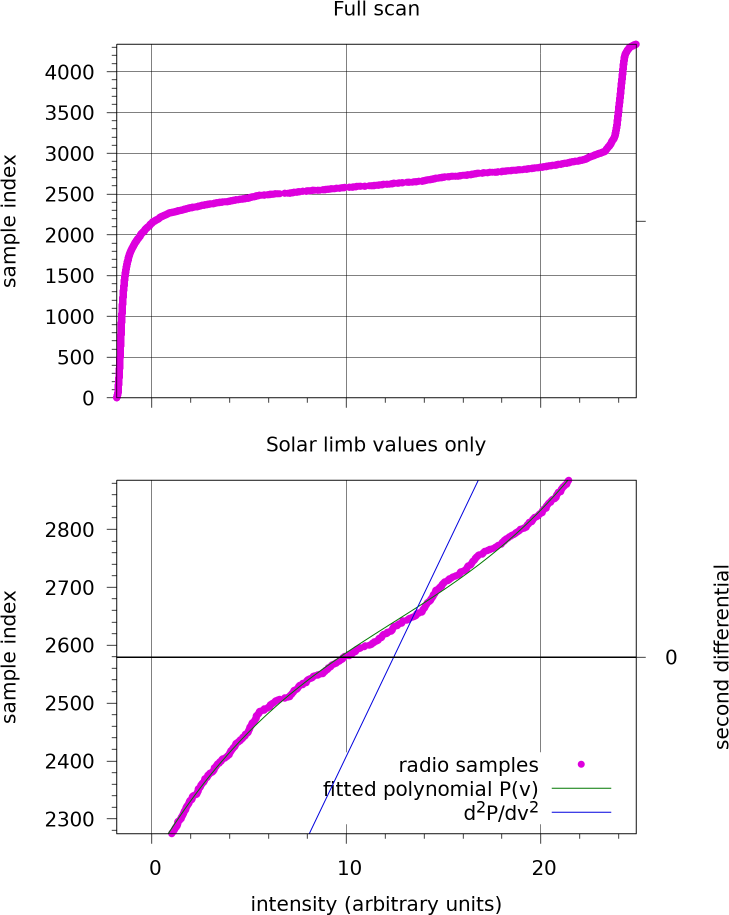
\includegraphics[width=8.5cm]{Scurve_example.png}
\caption{Radio samples of a typical solar scan sorted according to intensity. a) All samples. Between the dashed lines are the mixed samples which have contribution from the solar limb as well as the background. b) Only the mixed samples, into which a polynomial is fitted. A point of zero curvature (cross) provides a pivot point for signal level normalization.}
\label{S-curve_example}
\end{figure}

\fag{Suggestions: In general fonts in the plots are too small. They should at least be as large as the figure caption text. In figure\ref{S-curve_example}, make two plots stacked vertically with shared x-axis, so we can take advantage of the full column width.
Omit plot titles, these can be described in the captions. MJK: To me the labels look ok now. Perhaps you have already modified them according to Fred's suggestions. I am not so disturbed by the plot titles, but what is plotted in the different panels should be also explained in the figure caption. }

The sample $f_S(i_0)$ with index $i_0 := \floor{w(u_0)+0.5}$ is essentially in the middle of the disk boundary and provides pivot for signal level references. We set:
\eqnl{scurve-pivots}{
i_1 = \floor{\frac{i_0 + 1 + 1}{3} + 0.5} \quad \text{and} \quad i_2 = \floor{\frac{i_0 + |S|}{2} + 0.5} \text{.}
}
The intensity $w(i_1)$ then represents the background and $w(i_2)$ the quiet sun level (QSL). We then redo the polynomial fitting only for those samples which have intensity in the dynamic range of disk boundary, $10 .. 90 \%$ of QSL.
\eqnl{scurve-approx1}{
%MJK One line
%P^{(1)}(u) \approx w(u) \quad \text{for} \quad \frac{9 w(i_1) + w(i_2)}{10} \le u \le \frac{w(i_1) + 9 w(i_2)}{10} \text{.}
P^{(1)}(u) &\approx& w(u) \quad \text{for}\\ \quad \frac{9 w(i_1) + w(i_2)}{10} &\le& u \le \frac{w(i_1) + 9 w(i_2)}{10} \text{.} \nonumber
}
The result of this second fitting in shown in Figure \ref{S-curve_example}. We We find the roots:
\eqnl{scurve-roots1}{
%MJK One line
%u_1^{(1)} < ... < u_{n-2}^{(1)} 
&u_1^{(1)}& < ... < u_{n-2}^{(1)} \text{, for which} \quad \\
%MJK to remove space
%\quad 
%\text{, for which} \quad
&P^{(1)\prime\prime}(u_j^{(1)})& = 0 \text{, and} \quad 
u_0^{(1)} := u_{\frac{n-1}{2}}^{(1)} \nonumber 
}
%MJK indices?
and set pivot index
%MJK
as
%:
\eqnl{scurve-pivots1}{
%MJK One line
&i_0^{(1)}& := \floor{w(u_0^{(1)})+0.5}
%MJK comma
\text{,}
\quad i_1^{(1)} = \floor{\frac{i_0^{(1)} + 1 + 1}{3} + 0.5} 
%\quad 
%MJK comma
\text{,} 
%and} 
\nonumber \\
%\quad 
&i_2^{(1)}& = \floor{\frac{i_0^{(1)} + |S|}{2} + 0.5} \text{.}
}
We can now calibrate the intensity using $w(i_1^{(1)})$ for the background and $w(i_2^{(1)})$ for QSL:
\eqnl{scurve-calibration}{
s \in S \implies v(s) = \frac{u(s) - w(i_1^{(1)})}{w(i_2^{(1)}) - w(i_1^{(1)})} \text{.}
}

\subsection{Limb correction model}

We intend to estimate the brightness ($v$) based on time ($t$), heliographic latitude ($\theta$), angular distance from the 
%MJK comma '...disk, as seen...'
center of solar disk as seen at the time of observation ($r$), and the altitude above the horizon ($\varphi$). The model 
will contain polynomials of high degree, so that numerical stability is a concern. We need to carefully select the 
domains for each parameter. Radians are a natural choice of units for $\theta, \varphi \in \left( 0, \frac{\pi}{2} 
\right)$. For time, $t = \frac{a - 2005}{10}$, where $a$ is a real number $a = 1970 + 
\frac{\mathrm{unixtime}}{60\cdot60\cdot24\cdot365.25}$. Radius $r$ is represented as relative to the visual solar radius, which can 
either be calculated from our astronomical model or fitted to the data as a circle.


The solar map is a collection of intensity values $\left\{ v_i \right\}_i$ sampled by the antenna. These are linearly scaled so that $1$ represents the Quiet Sun Level (QSL) and $0$ represents the background. Each intensity value 
$v_i$ is accompanied with right ascension $\delta \mathrm{RA}_i$ and declination $\delta 
\mathrm{dec}_i$ relative to the center of the solar disk, $\left( \mathrm{RA}_{\mathrm{sun}}(t_i), 
\mathrm{dec}_{\mathrm{sun}}(t_i) \right)$, at the time of observation, $t_i$.


Moreover, $\varphi_i$ will be the altitude of the solar center at the time of observation, relative 
to observers horizon. It is measured in radians, and in practice samples will have the range:
\eqnl{altitude_range}{
\varphi_i \in \left[ \frac{5}{180} \pi, \frac{53}{180} \pi \right] \text{.}
}
Each sample also has weight $w_i$, which is set as to balance the target set. 
There are more 
observations starting from year $2015$, while only a few maps for year $1989$. 
%MJK Often we do just the opposite: if there are less data for a certain epoch, then the weigth is lower because of that time interval in more uncertain. Please expand on the logic here.
Thus we will put more weight on the old 
maps. Summer days typically have dozens of maps as the observational day is long, while on winter there are only a few maps per day.

We get more samples from the low heliographic latitudes, since a greater length of the solar equator is visible, 
compared to high latitude arcs. During summer, the solar north pole is visible to Earth, while we also get observations 
from high altitudes. During winter, we only observe the Sun at low altitude, and the solar south pole is visible. 
Further investigations are needed to exclude any bias effects arising from the unbalanced target set. However, having 
separate polynomials $P_n$ and $Q_m$ should reduce these risks. 
%MJK Good idea, but sounds like a task not necessary to undertake now? If the referee asks us to verify this risk, then we should do it. But, I comment it out for now...
%I suggest testing the optimization code with simulated 
%data.

%MJK The active region tracking tool is not yet described here. You are still planning to include that, right?

Limb intensity profiles showing brightening. 
\begin{figure}
\centering
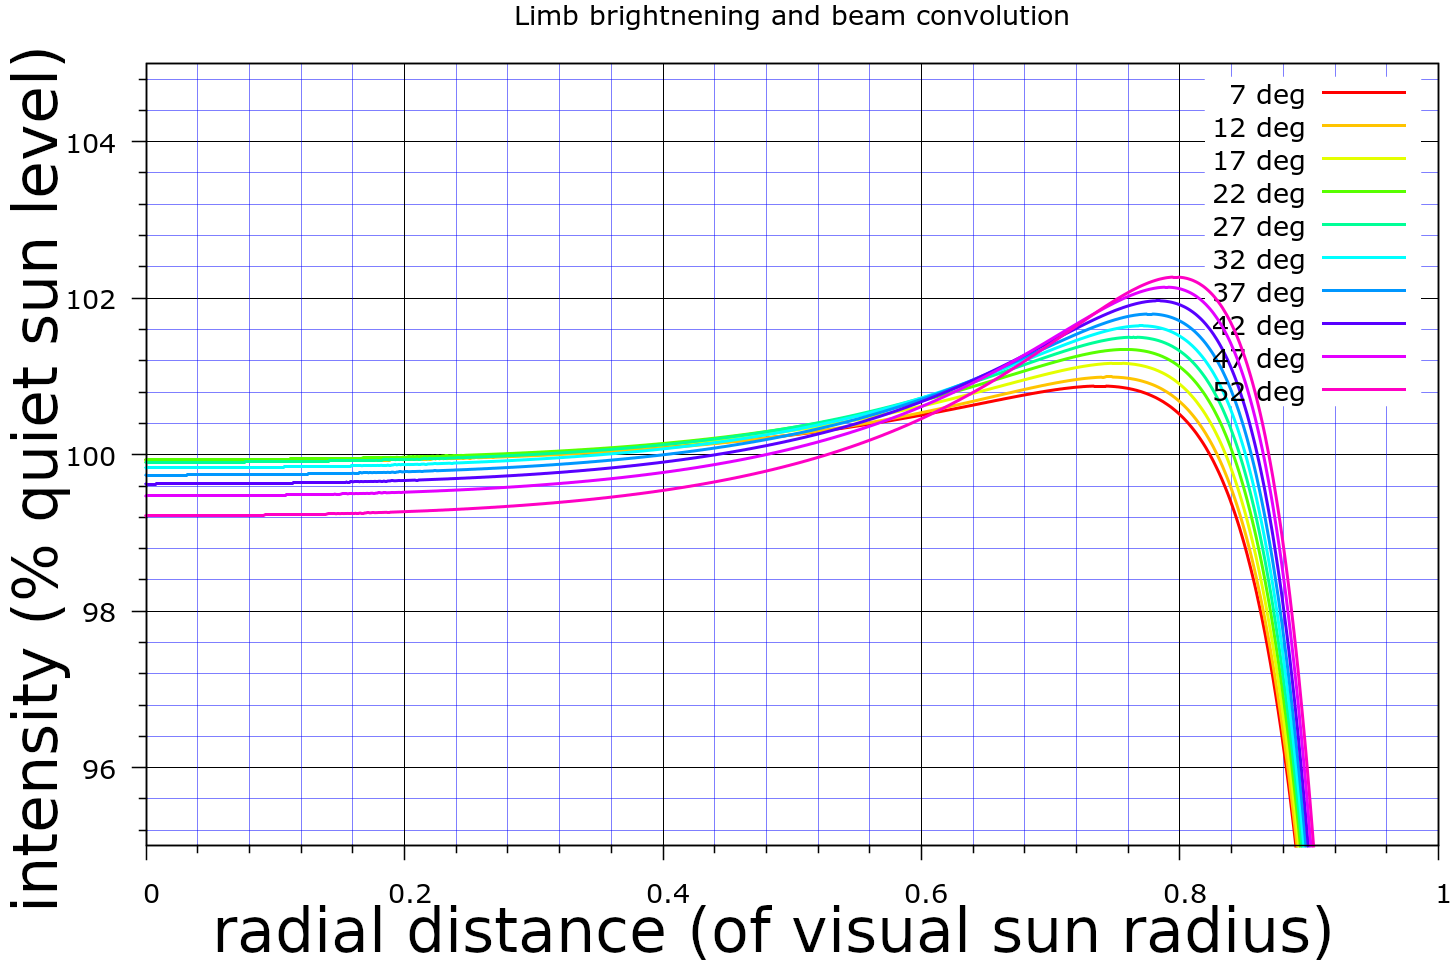
\includegraphics[width=8.5cm]{limbmodel_profiles1.png}
%MJK Here the axis labels now have huge (even too big) a font, while the label ticks still have quite a small font. Also, the legend box in the upper right corner overlaps with the data; can it be placed, e.g., in the upper left corner?
\caption{Limb intensity profiles showing brightening. When observed at low altitudes, the profiles are significantly blurred. Comment: fix font sizes.}
\label{limb_brightening1}
\end{figure}

\begin{figure}
\centering
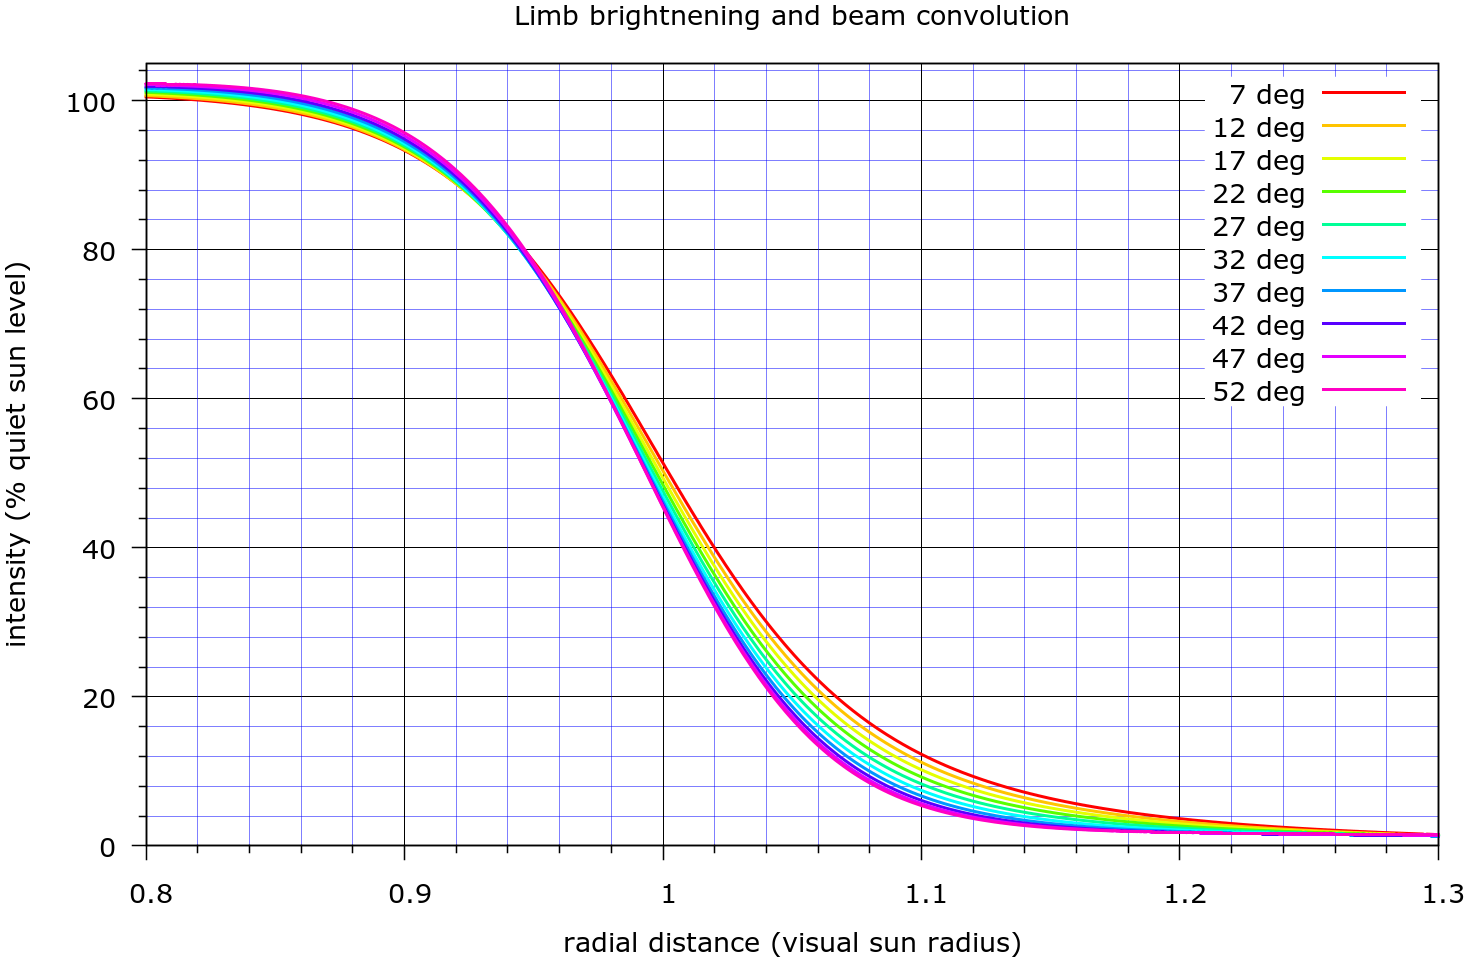
\includegraphics[width=8.5cm]{limbmodel_profiles2.png}
%MJK Too small axis labels and ticks.
\caption{Limb intensity profiles with convolution effects. Comment: Fix font sizes.}
\label{limb_brightening2}
\end{figure}

\begin{figure*}
\centering
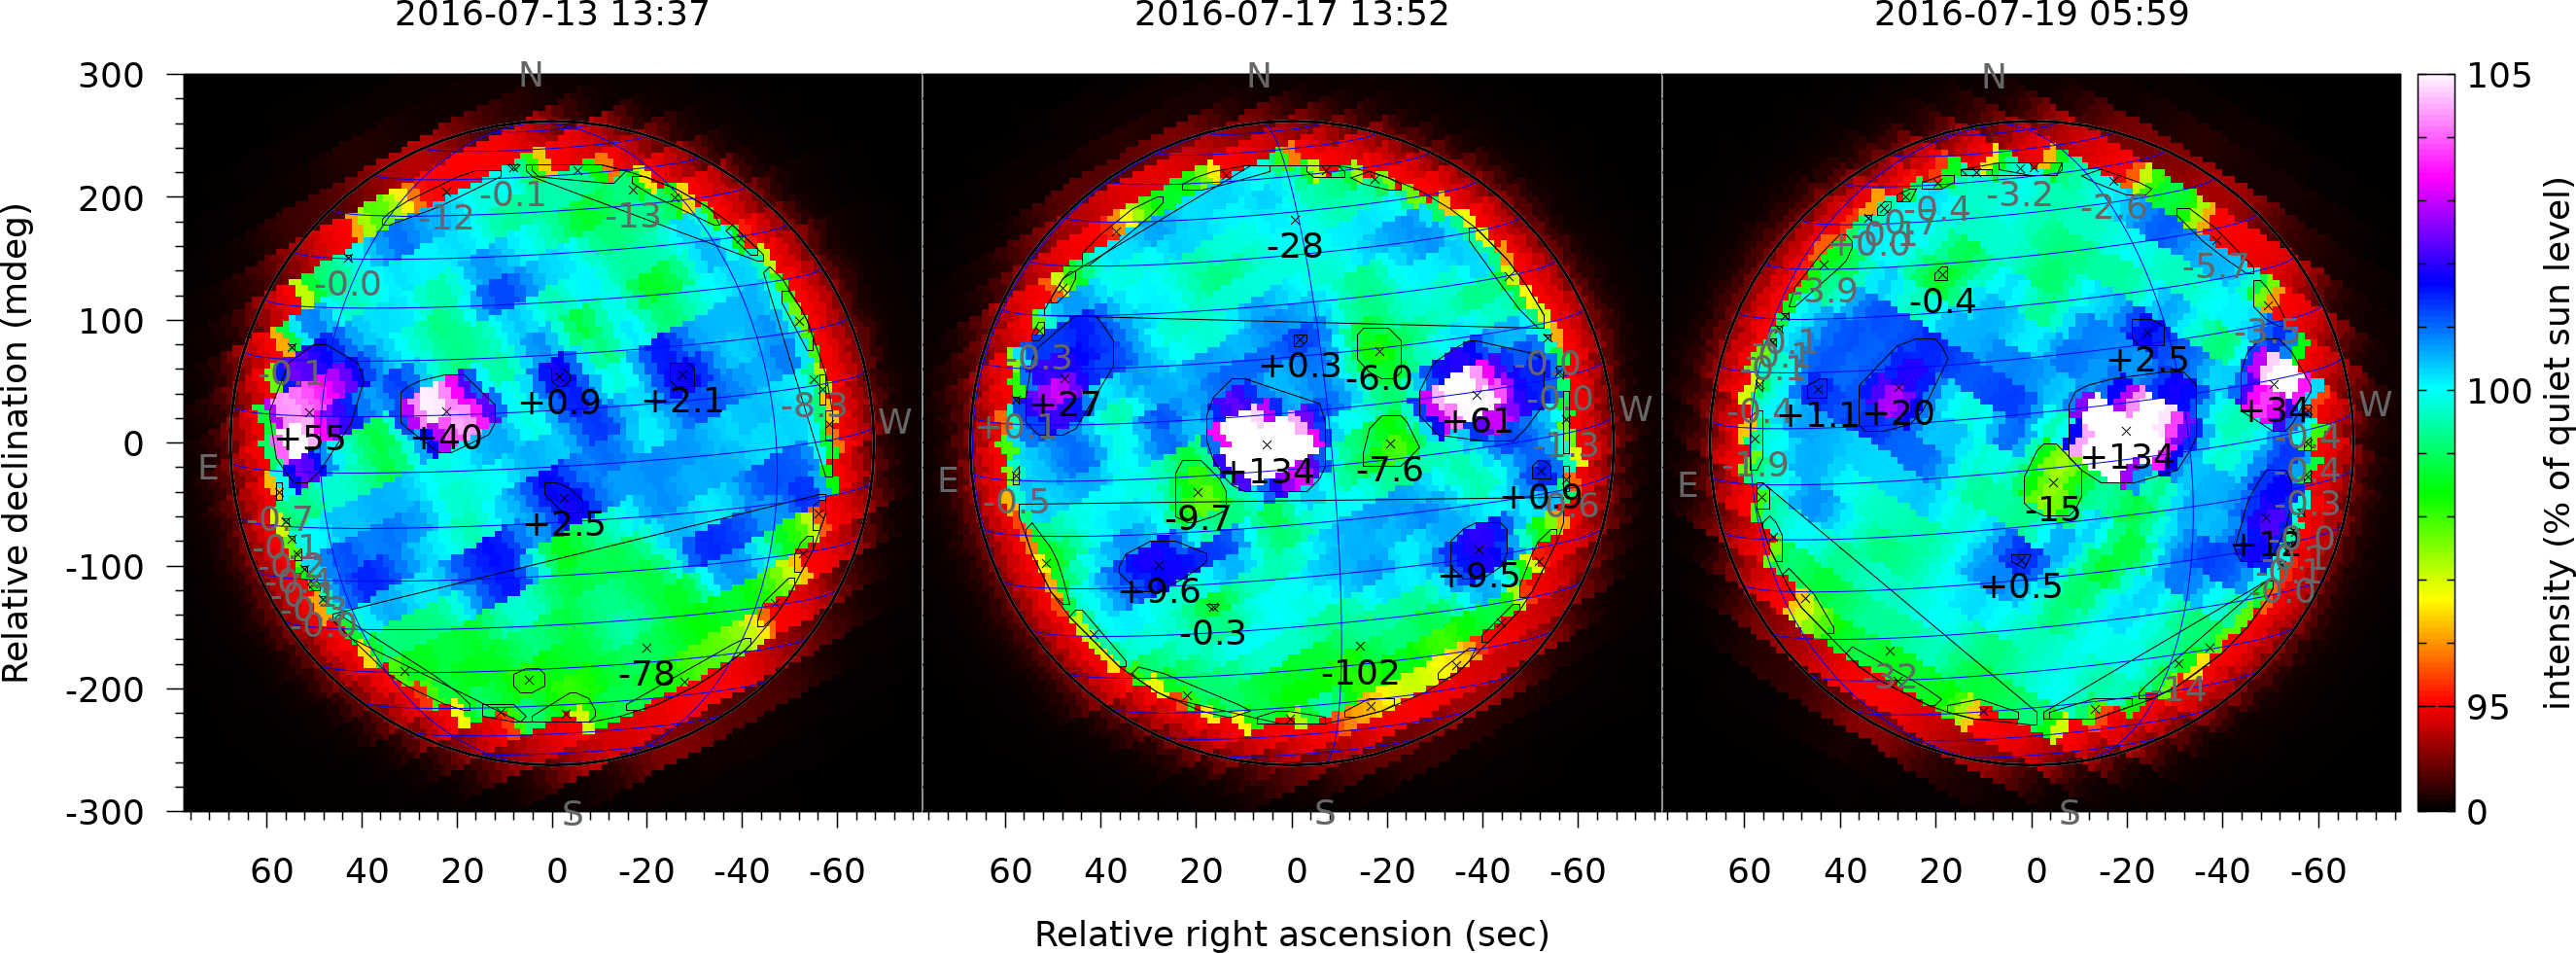
\includegraphics[width=\textwidth]{maptrack1.png}
\caption{Two active regions passing the visible disk as the Sun rotates.}
\label{maptrack1}
\end{figure*}

\begin{figure} \centering 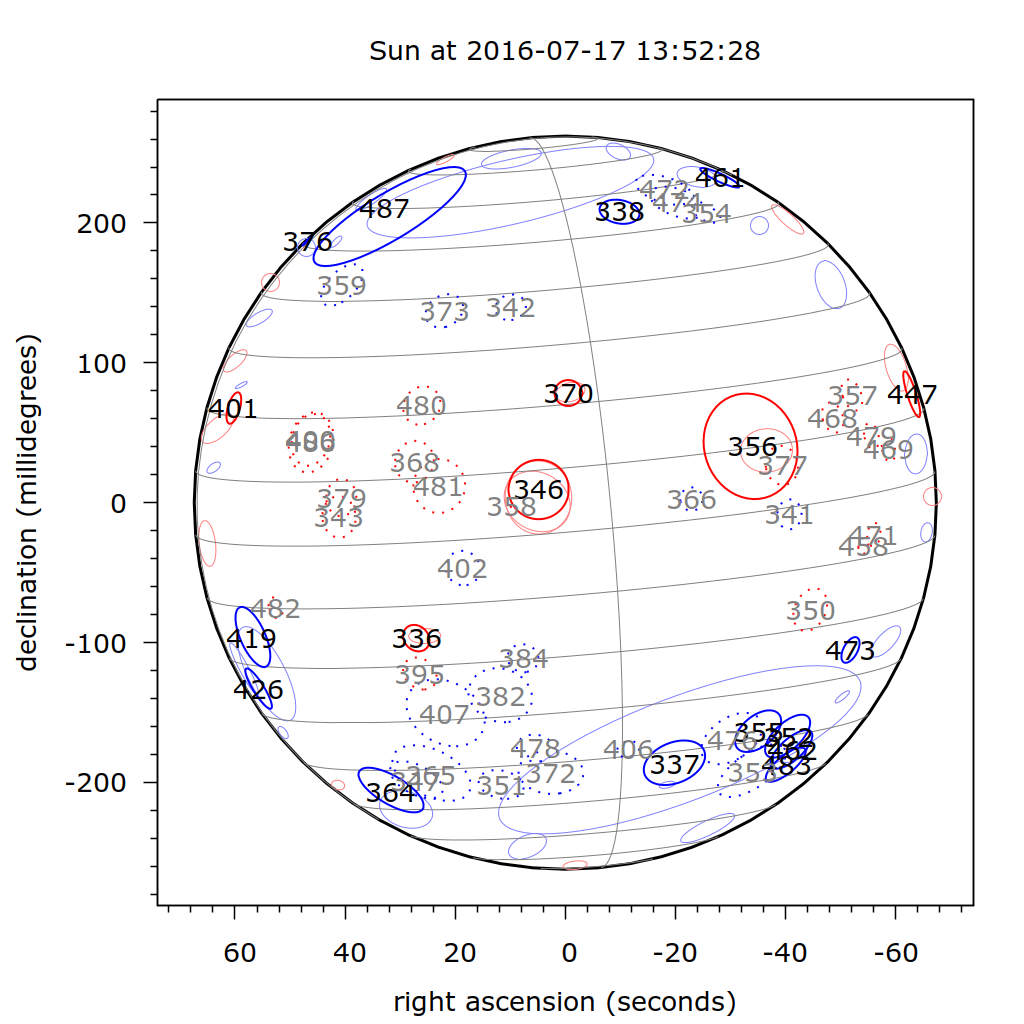
\includegraphics[width=8.8cm]{maptrack2.png} \caption{Tracked regions are shown with red 
ellipses for bright regions and with blue ellipses for dim regions. Based on earlier and later sunmaps, we can often 
expect a weak region to be visible at known heliographic coordinates. When the region nevertheless is found on this map, 
we show it with a dashed ellipse. The active regions 346 and 356 are clearly visible in Figure \ref{maptrack1}.} 
\label{maptrack2} \end{figure}


%\begin{figure}
%\centering
%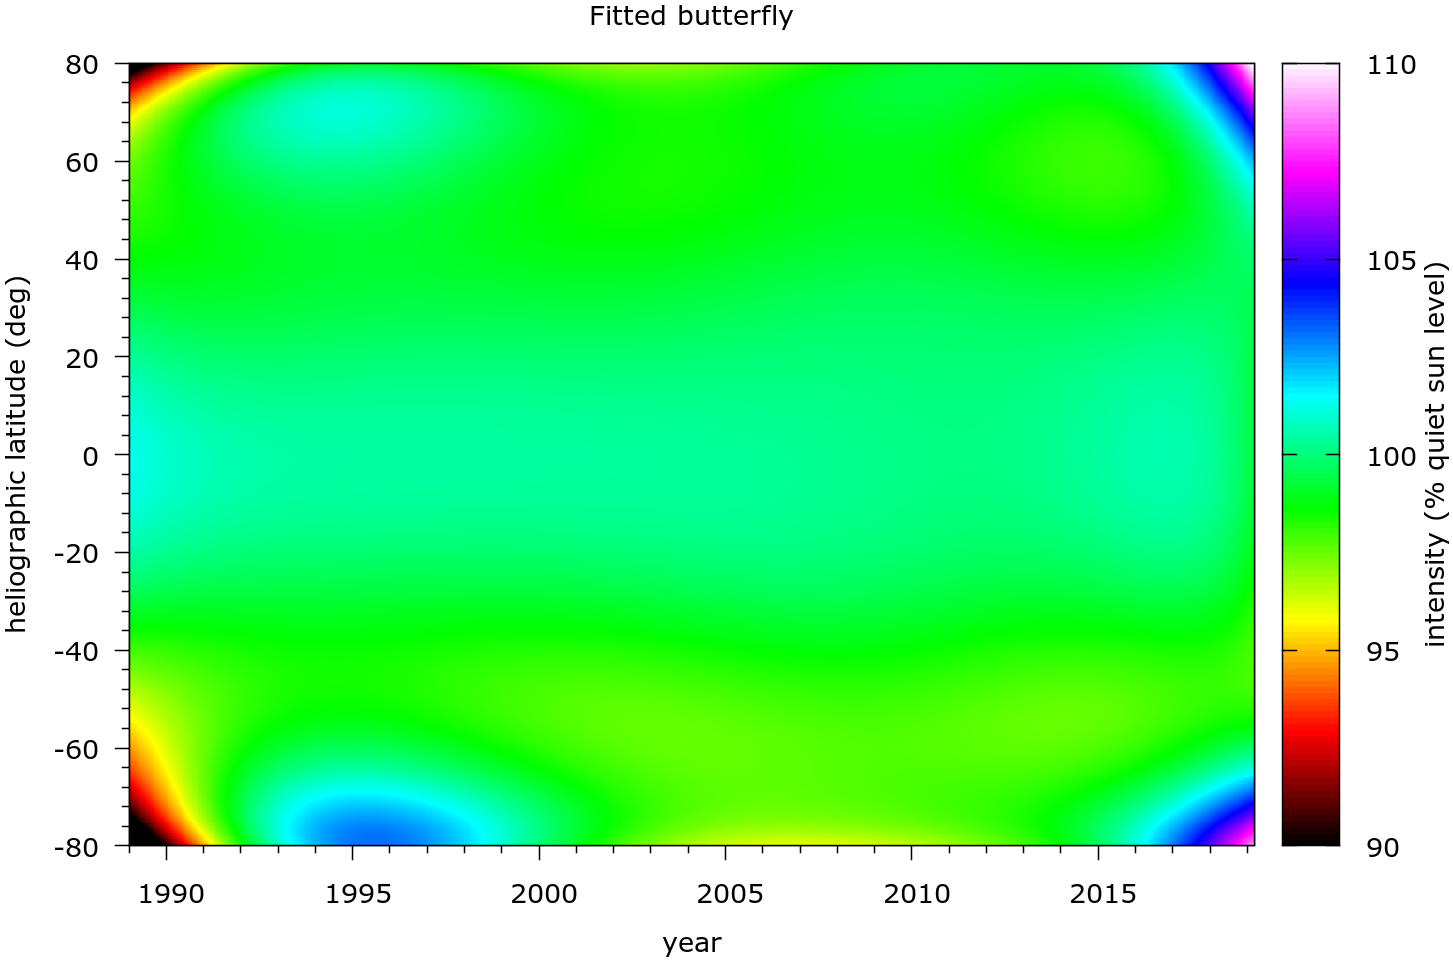
\includegraphics[width=8.5cm]{limbmodel_butterfly1.png}
%\caption{Idealized butterfly diagram showing cyclic behaviour at high %latitudes.}
%\label{limb_butterfly1}
%\end{figure}

%\begin{figure}
%\centering
%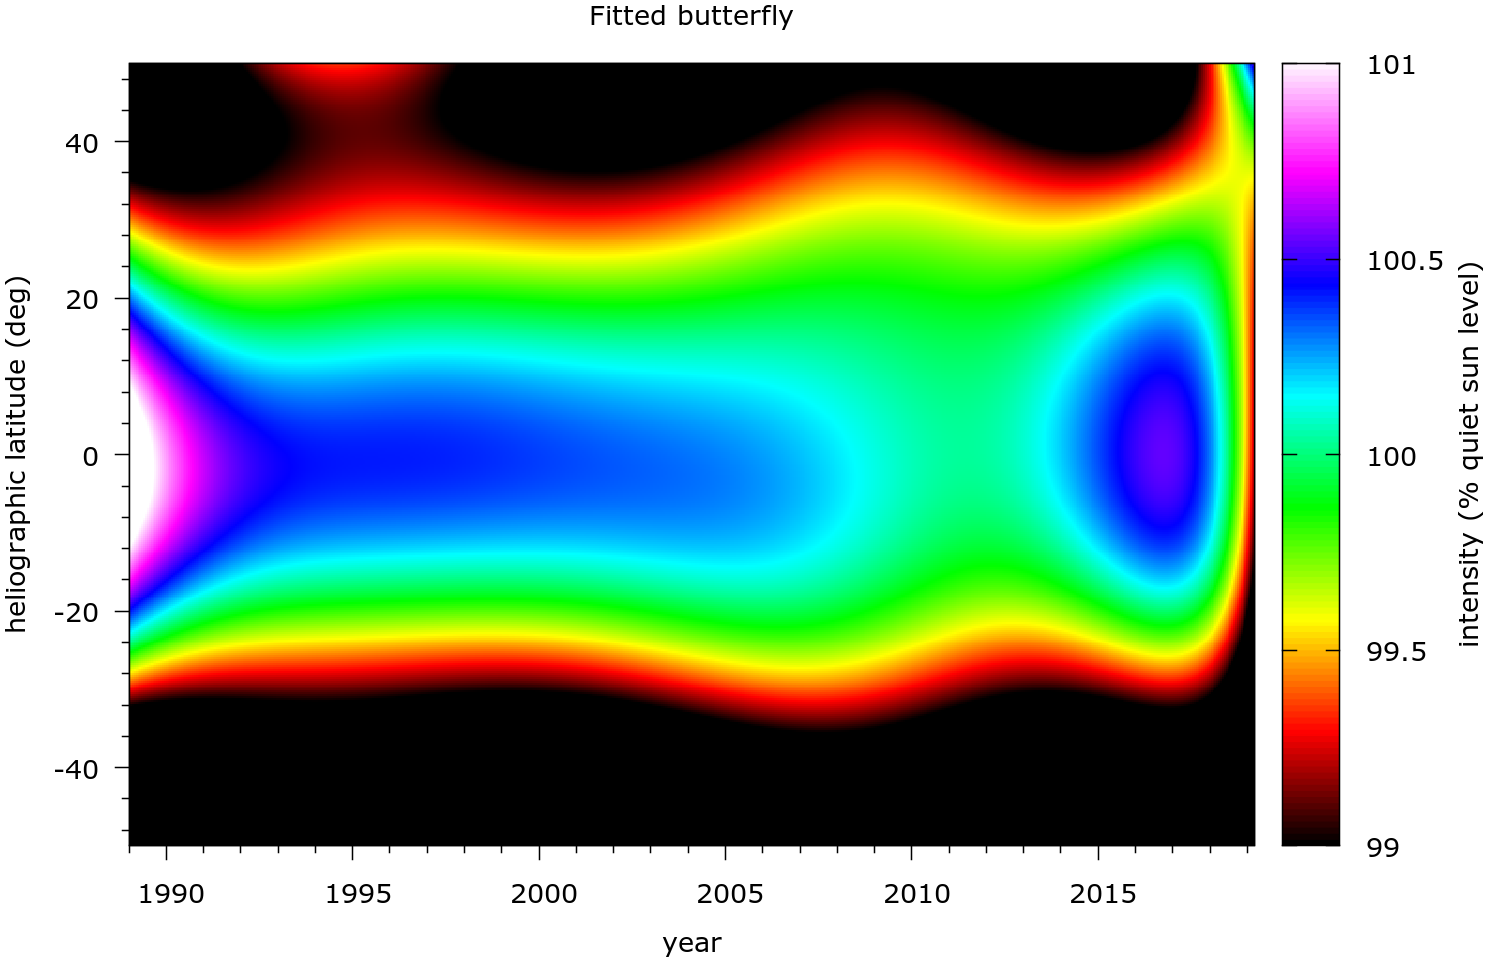
\includegraphics[width=8.5cm]{limbmodel_butterfly2.png}
%\caption{Idealized butterfly diagram with emphasis on the low %latitudes.}
%\label{limb_butterfly2}
%\end{figure}

\begin{figure}
\centering
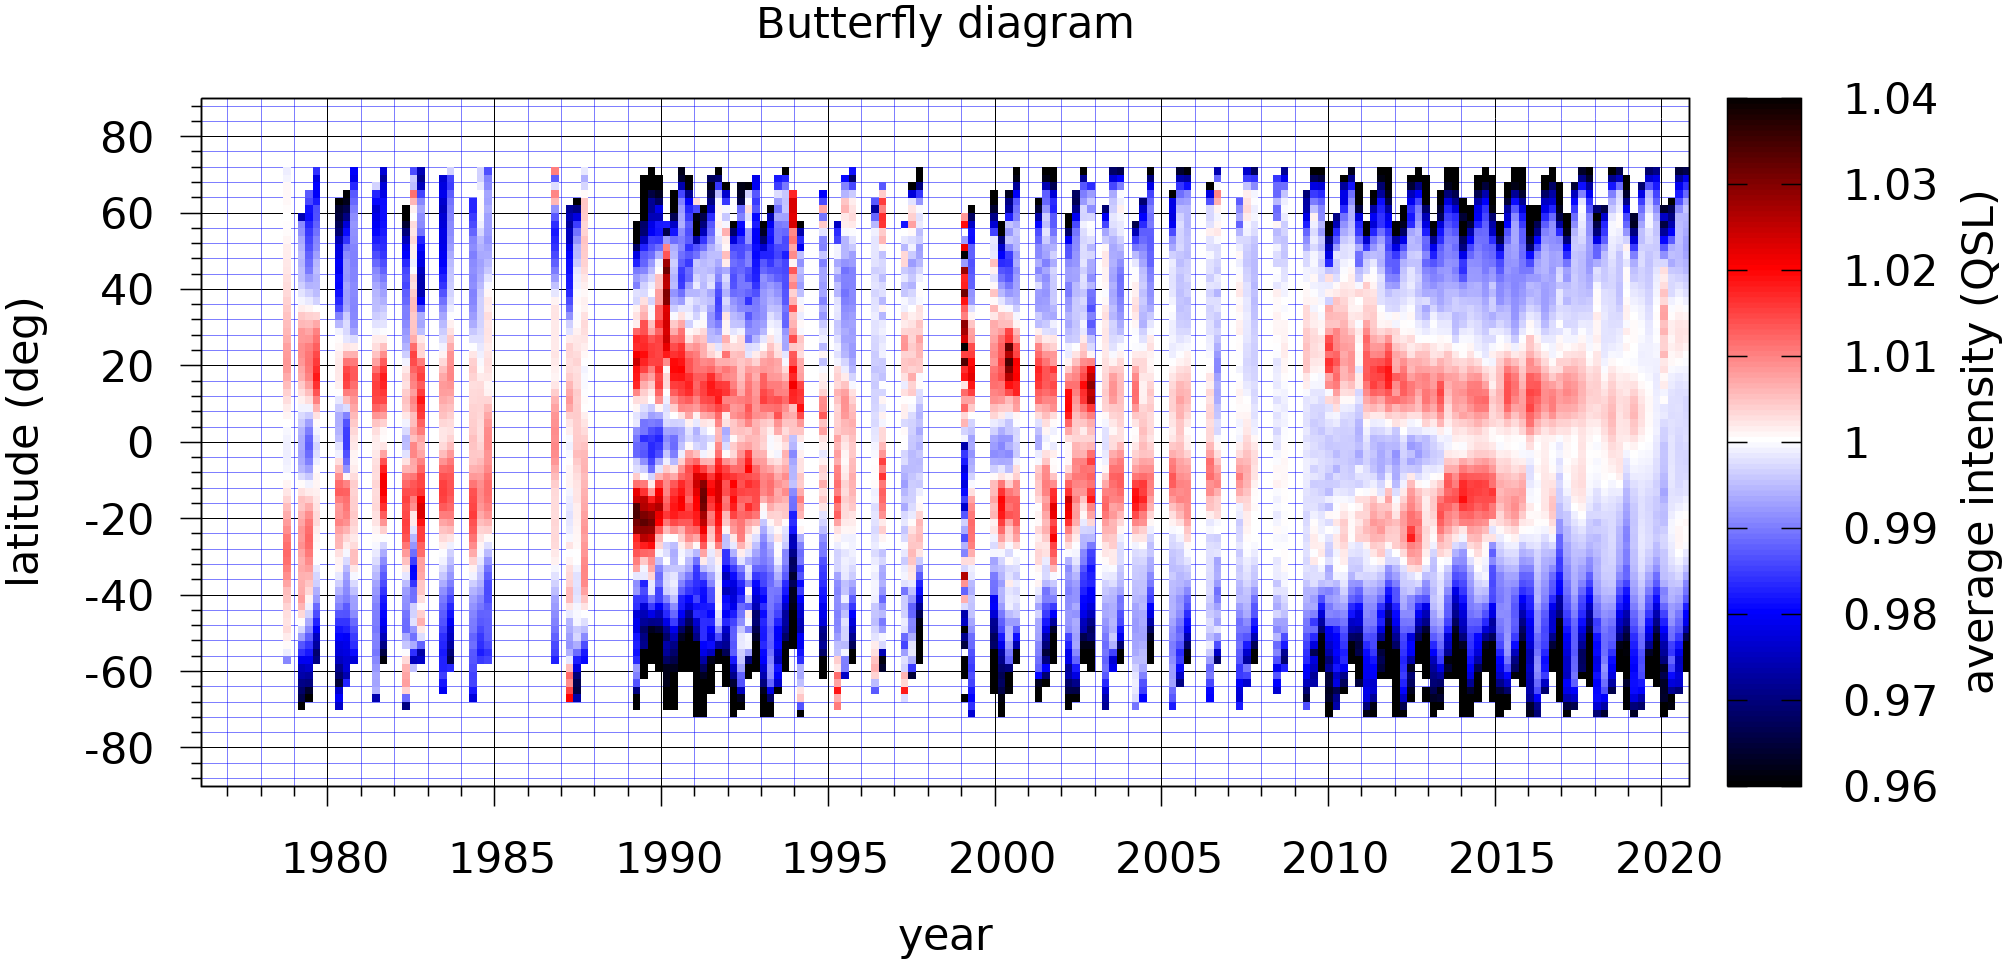
\includegraphics[width=8.5cm]{butterfly_clear_raw.png}
\caption{Solar intensity at all heliographic latitudes on $\si{37}{GHz}$ over cycles 21 to 24. Averaged over samples for which $r_i \le 0.9$ to avoid beam mixing with the background.
}
\label{butterfly_clear_raw}
\end{figure}
\fag{(later) obtain same period of photospheric sunspot numbers
Tabulate the timespans and line fits for all eight.}\\

\begin{figure}
\centering
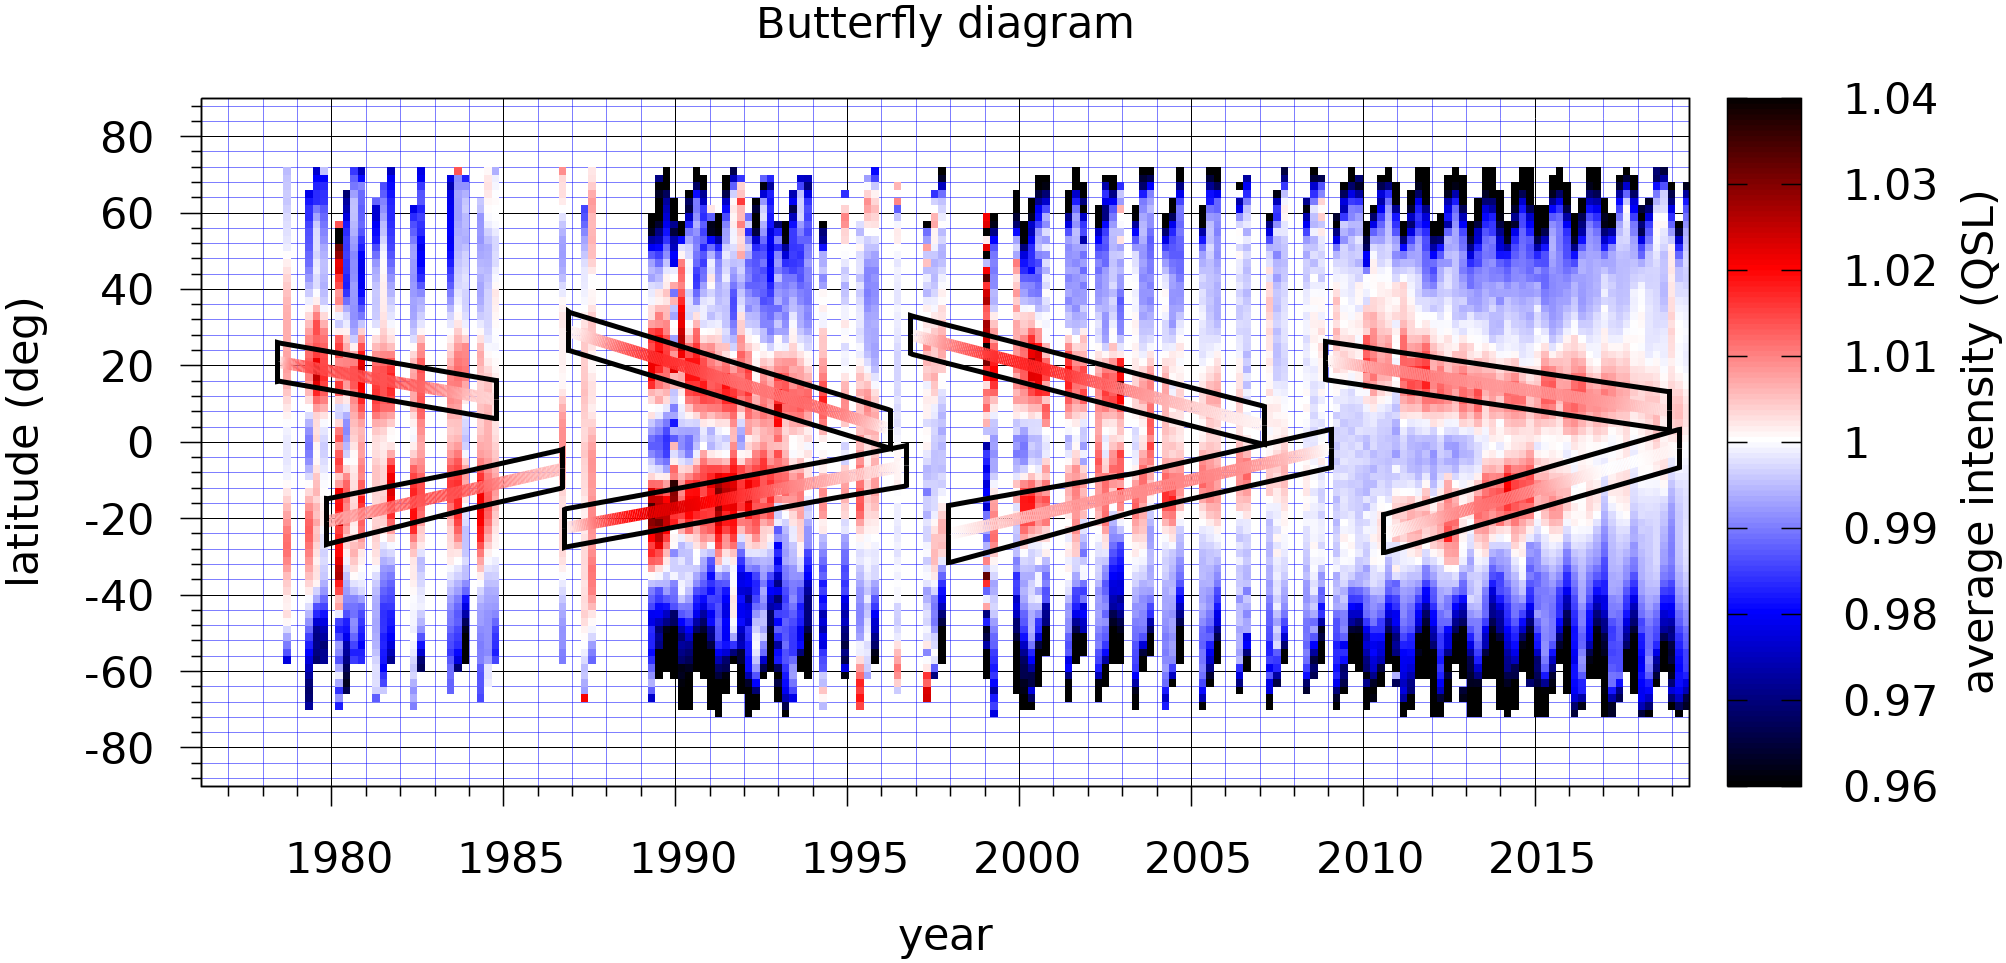
\includegraphics[width=8.5cm]{butterfly_wingfit_raw.png}
\caption{Butterfly wing patterns automatically fitted on top of Mets\"ahovi $\SI{37}{GHz}$ data (cf. Figure \ref{butterfly_clear_corr}).} 
\label{butterfly_wingfit_raw}
\end{figure}

\begin{figure}
\centering
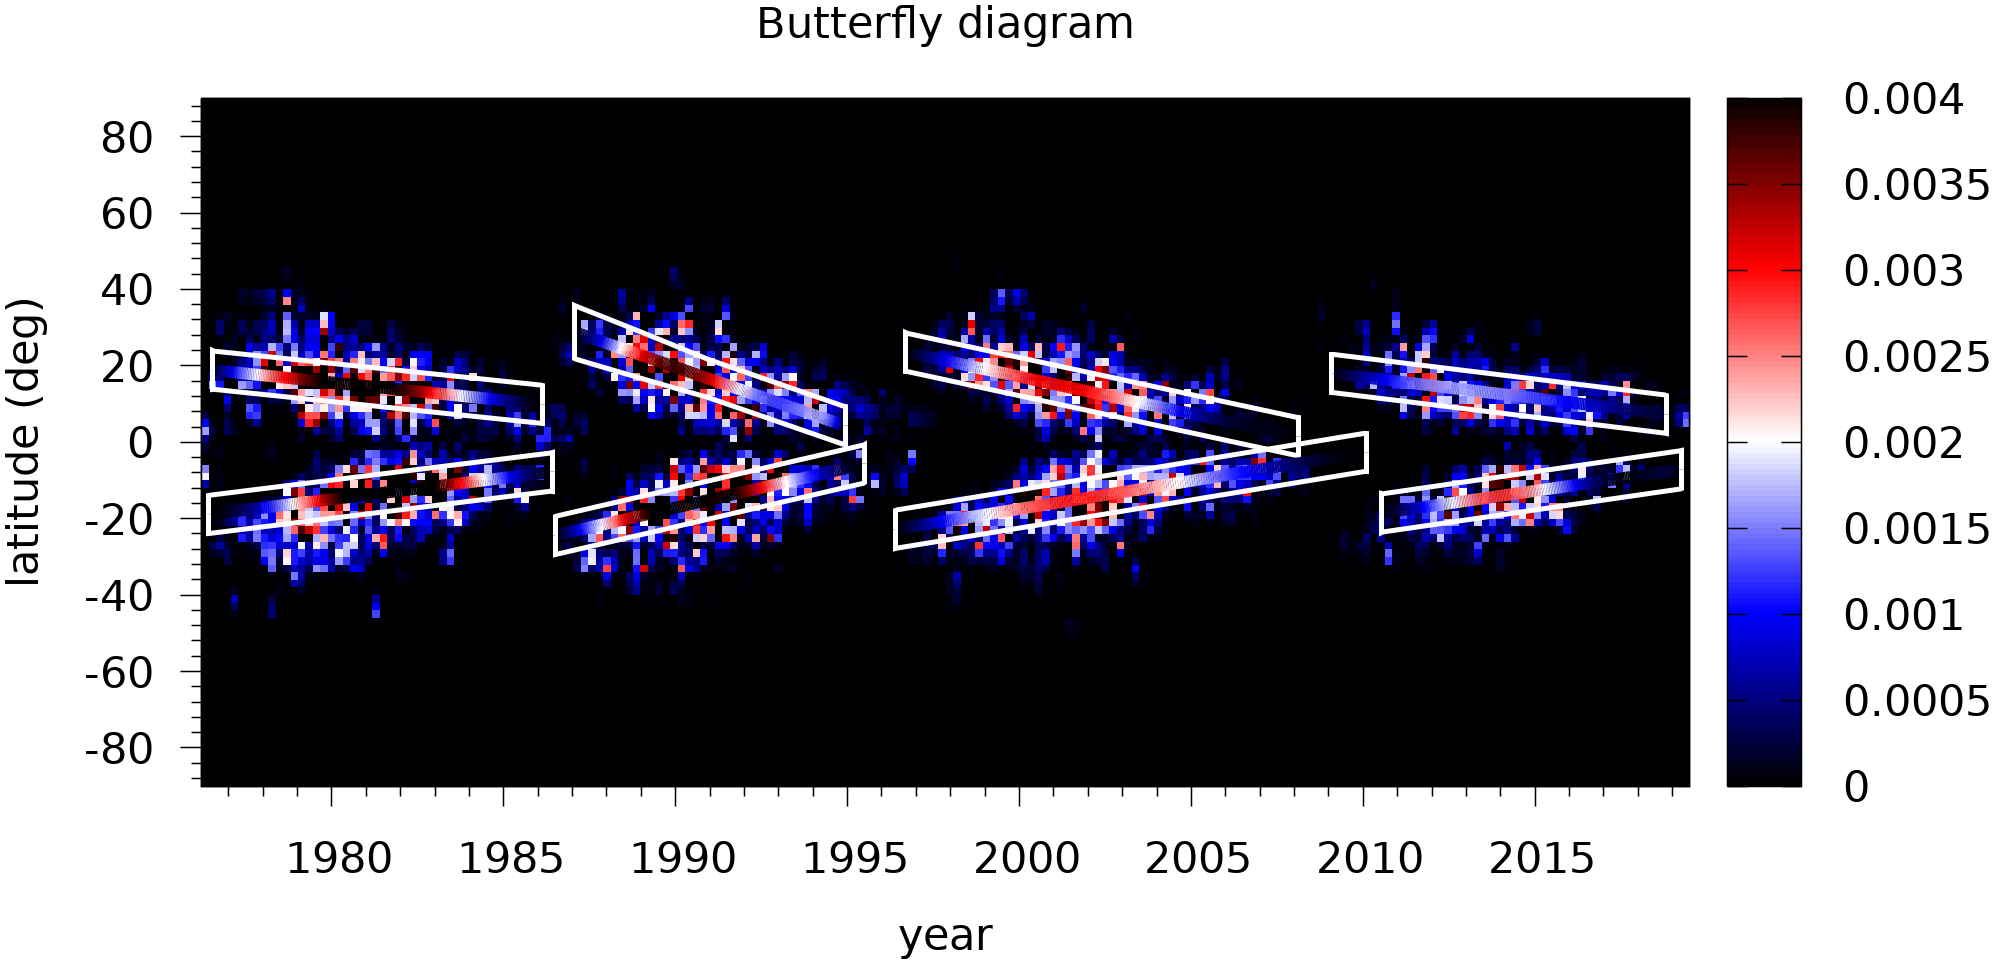
\includegraphics[width=8.5cm]{butterfly_wingfit_sunspot.png}
\caption{Butterfly wing patterns automatically fitted on sunspot data \cite{SUNSPOTDATA:1}. The sunspot cycle coincides with the radio cycle seen in Figure. \ref{butterfly_wingfit_raw}. Comment: fix 21st cycle fitting.}
\label{butterfly_wingfit_sunspot}
\end{figure}

\begin{figure}
\centering
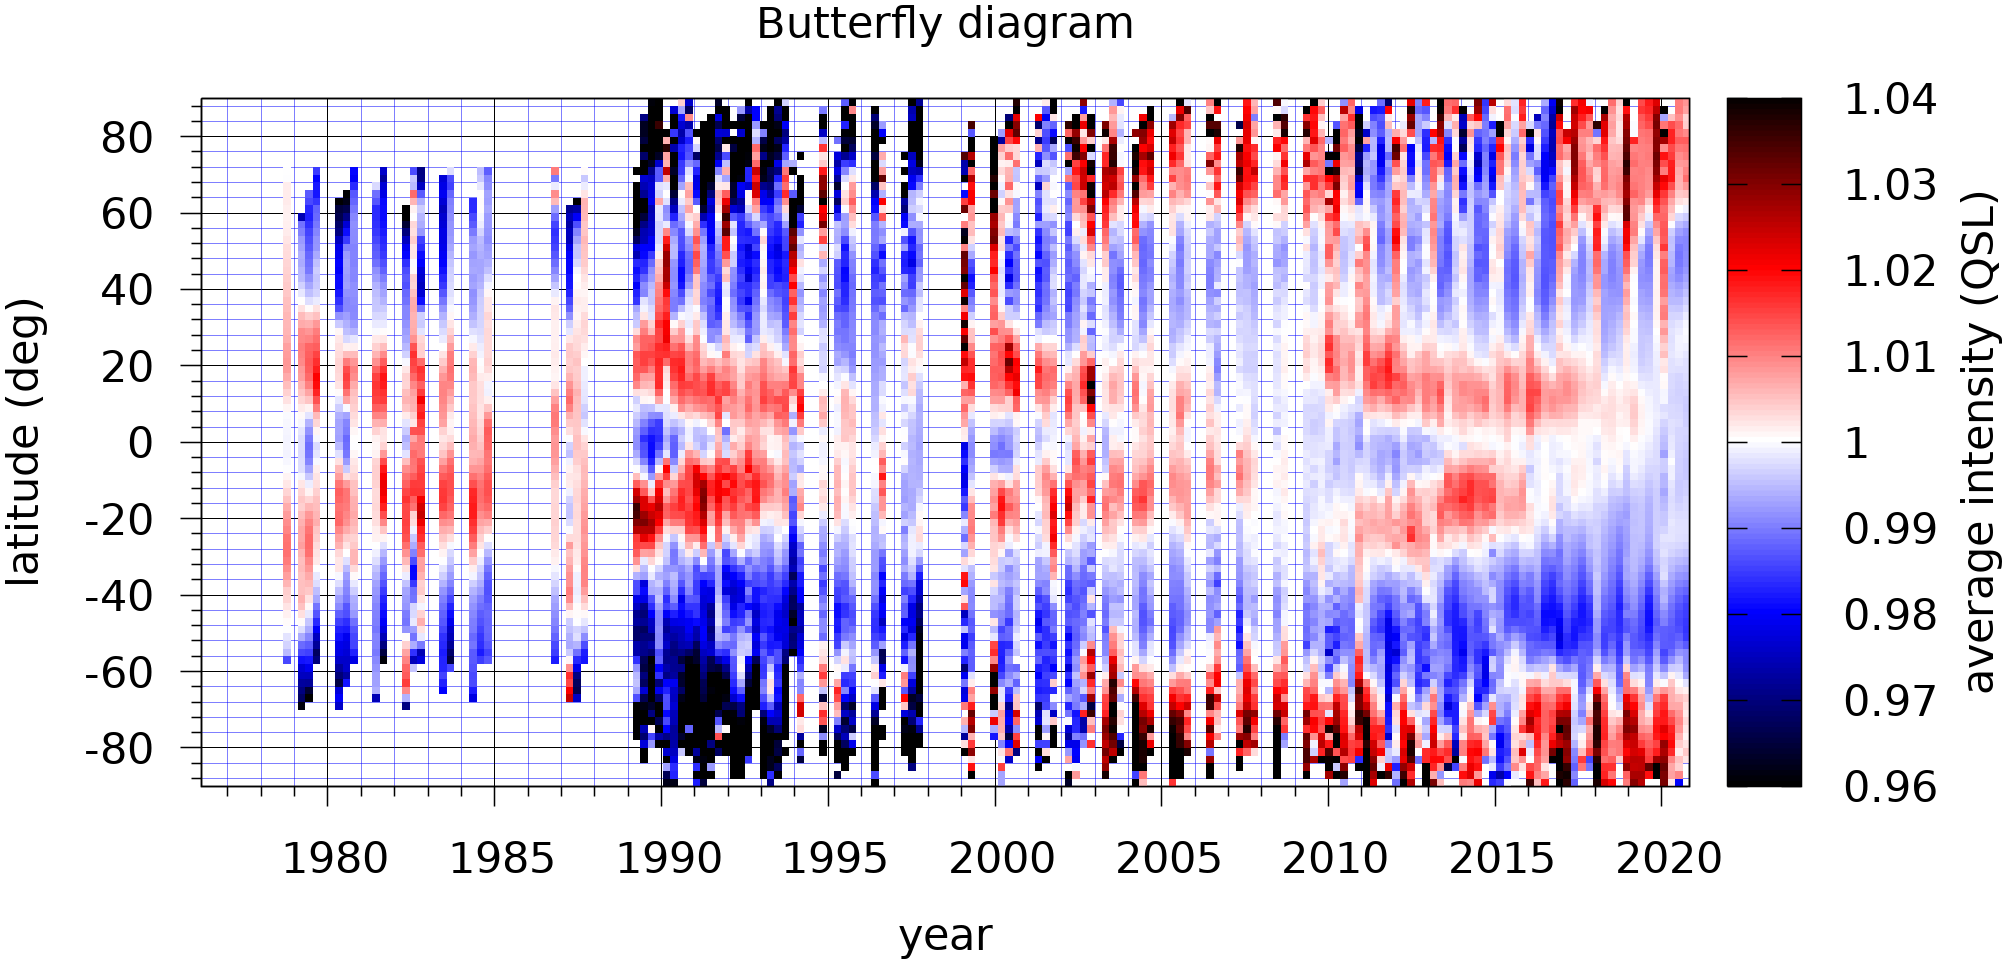
\includegraphics[width=8.5cm]{butterfly_clear_limb.png}
\caption{Solar intensity at all heliographic latitudes on $\si{37}{GHz}$ over cycles 21 to 24. Averaged over samples for which $r_i \le 1.0$ so that each sample intensity is corrected for beam mixing and limb brightening. This increases the available latitude range, bringing the polar magnetic cycle clearly visible.}
\label{butterfly_clear_corr}
\end{figure}

%-------------------------------------- Two column figure (place early!)




\section{Results}\label{sect:results}
\fag{To do identify other observations/publications on polar magnetic cycles to compare with
Figure\,\ref{butterfly_clear_corr}. MJK: The Srivastava et al., 2018 paper should give plenty of refences. And perhaps more references can be found from those papers.}\\

\begin{table}
\caption{\label{tab:cycles}
Heliographic solar intensity butterfly fits for cycles 21 -- 24, by hemisphere.
Latitude Lat$_0$ and time $t_0$ at the start of each cycle, the slope of transition
towards the Equator, the time $t_{\rm end}$ at which each cycle is considered to have
ceased and the length of each cycle $\tau_{\rm cycle}$.
}
\begin{tabular}{l|ccccr}
\hline\hline
Cycle & Lat ($t_0$) & $t_0$ & slope                   & $t_{\rm end}$   & $	\tau_{\rm cycle}$ \\
      & [$\deg$]      &  [yr] & [$\deg{\rm yr}^{-1}$]   & [yr]            & [yr]                \\
\hline \\
21N & $+18.5^{\circ}$ & $1977.8$ & $-0.6$ & $1987.1$ &  9.3 \\
21S & $-19.1^{\circ}$ & $1979.3$ & $+1.8$ & $1986.8$ &  7.5 \\
\\
22N & $+31.0^{\circ}$ & $1987.1$ & $-3.0$ & $1996.7$ &  9.6 \\
22S & $-22.8^{\circ}$ & $1984.9$ & $+1.3$ & $1996.0$ & 11.1 \\
\\
23N & $+28.5^{\circ}$ & $1996.6$ & $-2.2$ & $2005.9$ &  9.3 \\
23S & $-25.4^{\circ}$ & $1998.2$ & $+2.4$ & $2008.4$ & 10.2 \\
\\
24N & $+21.6^{\circ}$ & $2008.2$ & $-1.2$ & $2019.5$ & 11.3 \\
24S & $-23.8^{\circ}$ & $2010.2$ & $+2.3$ & $2017.4$ &  7.1 \\
\\

\hline
\end{tabular}
\end{table}

\begin{table}
\caption{\label{tab:cycles_sunspot}
Sunspot data fits for cycles 21 -- 24, by hemisphere.
Latitude Lat$_0$ and time $t_0$ at the start of each cycle, the slope of transition
towards the Equator, the time $t_{\rm end}$ at which each cycle is considered to have
ceased and the length of each cycle $\tau_{\rm cycle}$.
}
\begin{tabular}{l|ccccr}
\hline\hline
Cycle & Lat ($t_0$) & $t_0$ & slope                   & $t_{\rm end}$   & $	\tau_{\rm cycle}$ \\
      & [$\deg$]      &  [yr] & [$\deg{\rm yr}^{-1}$]   & [yr]            & [yr]                \\
\hline \\
21N & $+17.5^{\circ}$ & $1977.6$ & $-0.8$ & $1985.6$ &  8.0 \\
21S & $-14.6^{\circ}$ & $1978.1$ & $+0.6$ & $1986.3$ &  8.3 \\
\\
22N & $+32.6^{\circ}$ & $1986.8$ & $-3.9$ & $1994.3$ &  7.5 \\
22S & $-24.1^{\circ}$ & $1986.4$ & $+2.1$ & $1994.8$ &  8.4 \\
\\
23N & $+24.3^{\circ}$ & $1996.5$ & $-1.9$ & $2006.3$ &  9.8 \\
23S & $-23.6^{\circ}$ & $1995.9$ & $+1.5$ & $2008.6$ & 12.7 \\
\\
24N & $+17.8^{\circ}$ & $2008.7$ & $-1.0$ & $2018.5$ &  9.8 \\
24S & $-18.9^{\circ}$ & $2010.3$ & $+1.4$ & $2017.8$ &  7.5 \\
\\

\hline
\end{tabular}
\end{table}

%
%\begin{figure*}
%\centering
%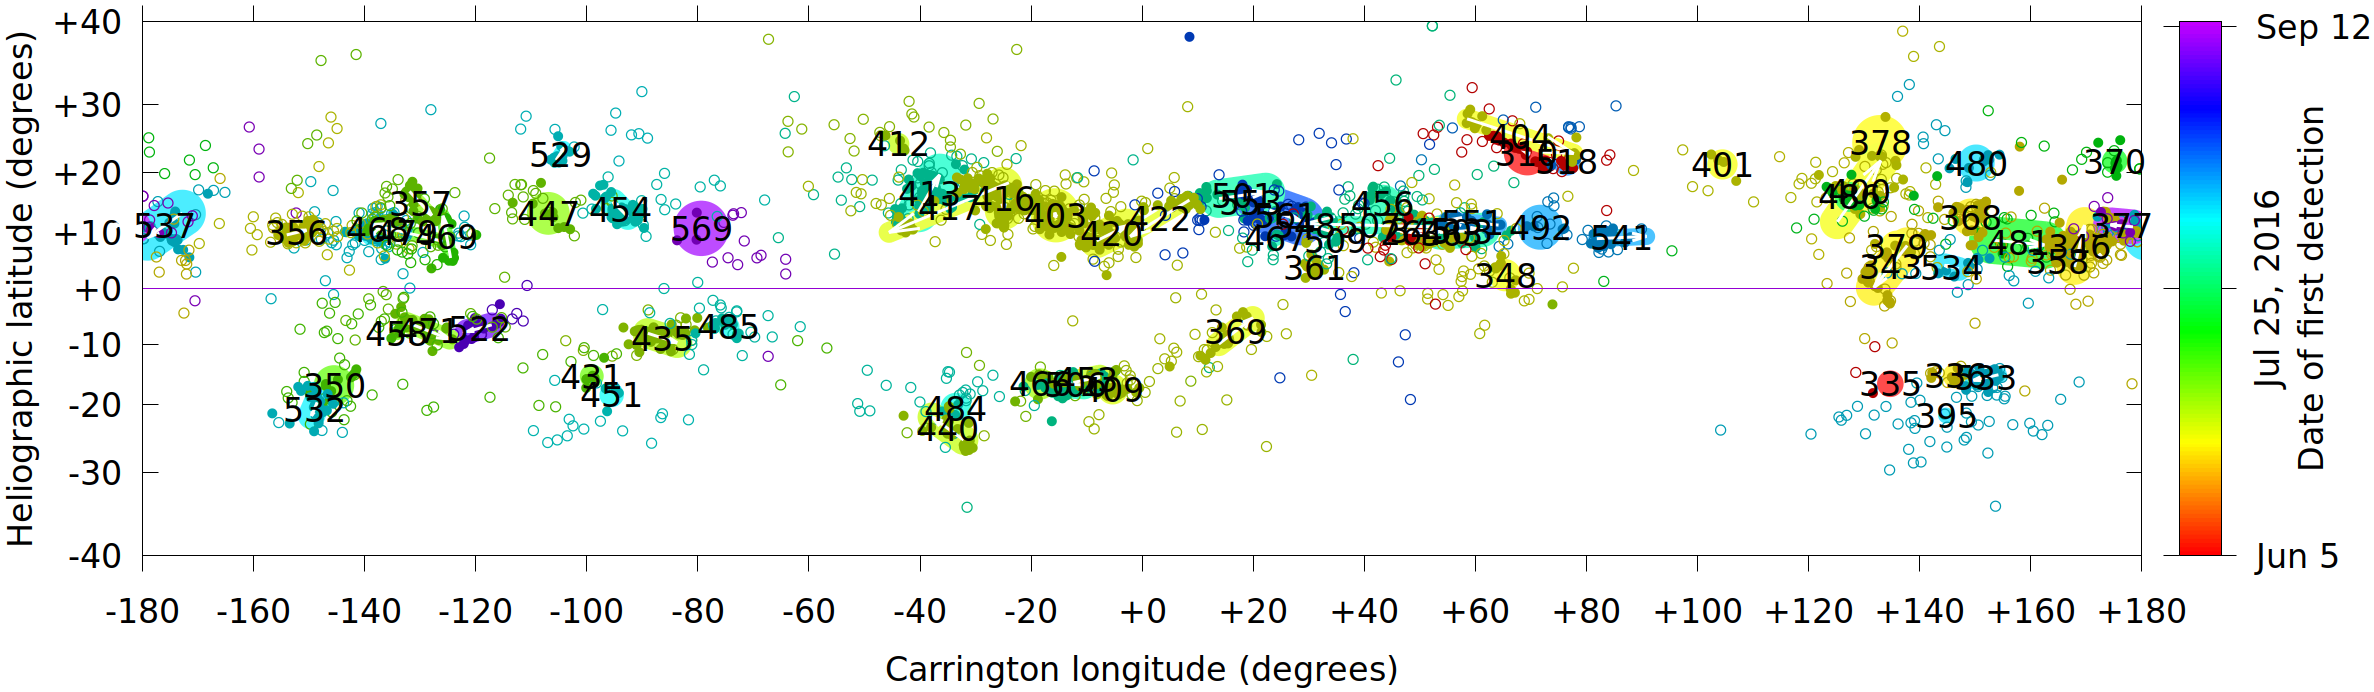
\includegraphics[width=18.5cm]{carrington1.png}
%\caption{Heliographic map showing tracked regions.}
%\label{carrington1}
%\end{figure*}
%
%\begin{figure}
%\centering
%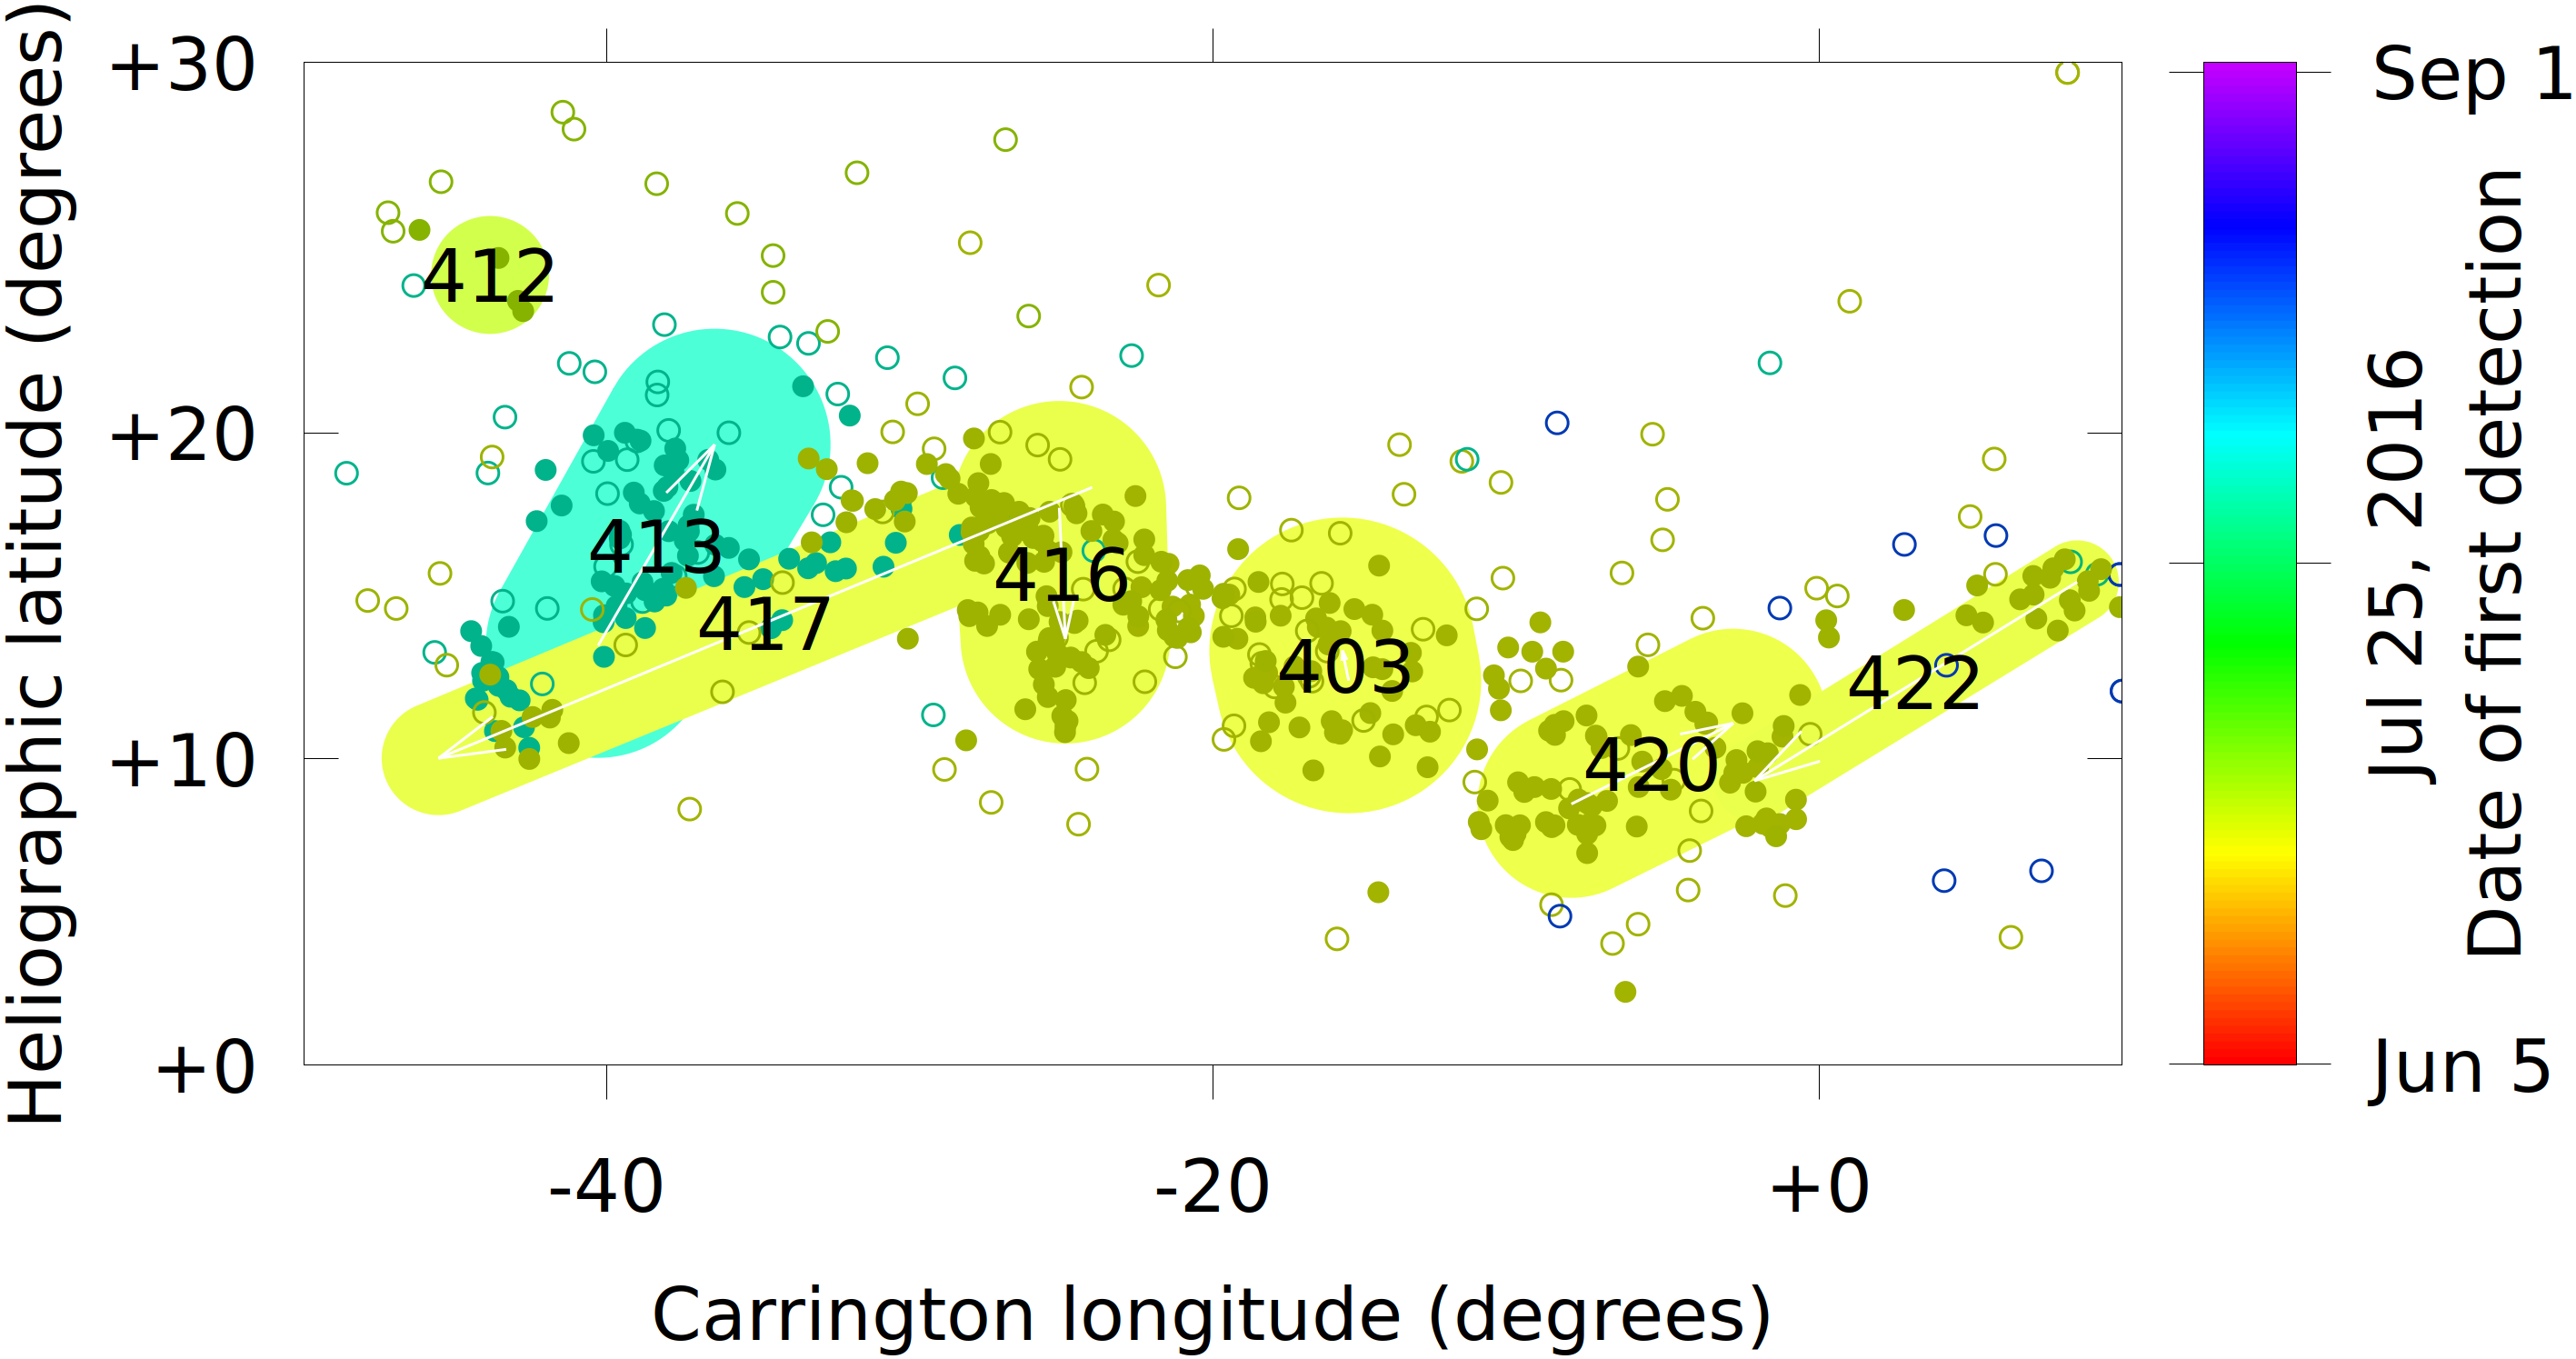
\includegraphics[width=8.8cm]{carrington2.png}
%\caption{Closeup of Figure \ref{carrington1} showing details of individual tracks. Migration during the given time interval is represented with arrows.}
%\label{carrington2}
%\end{figure}
%
%
%\begin{figure}
%\centering
%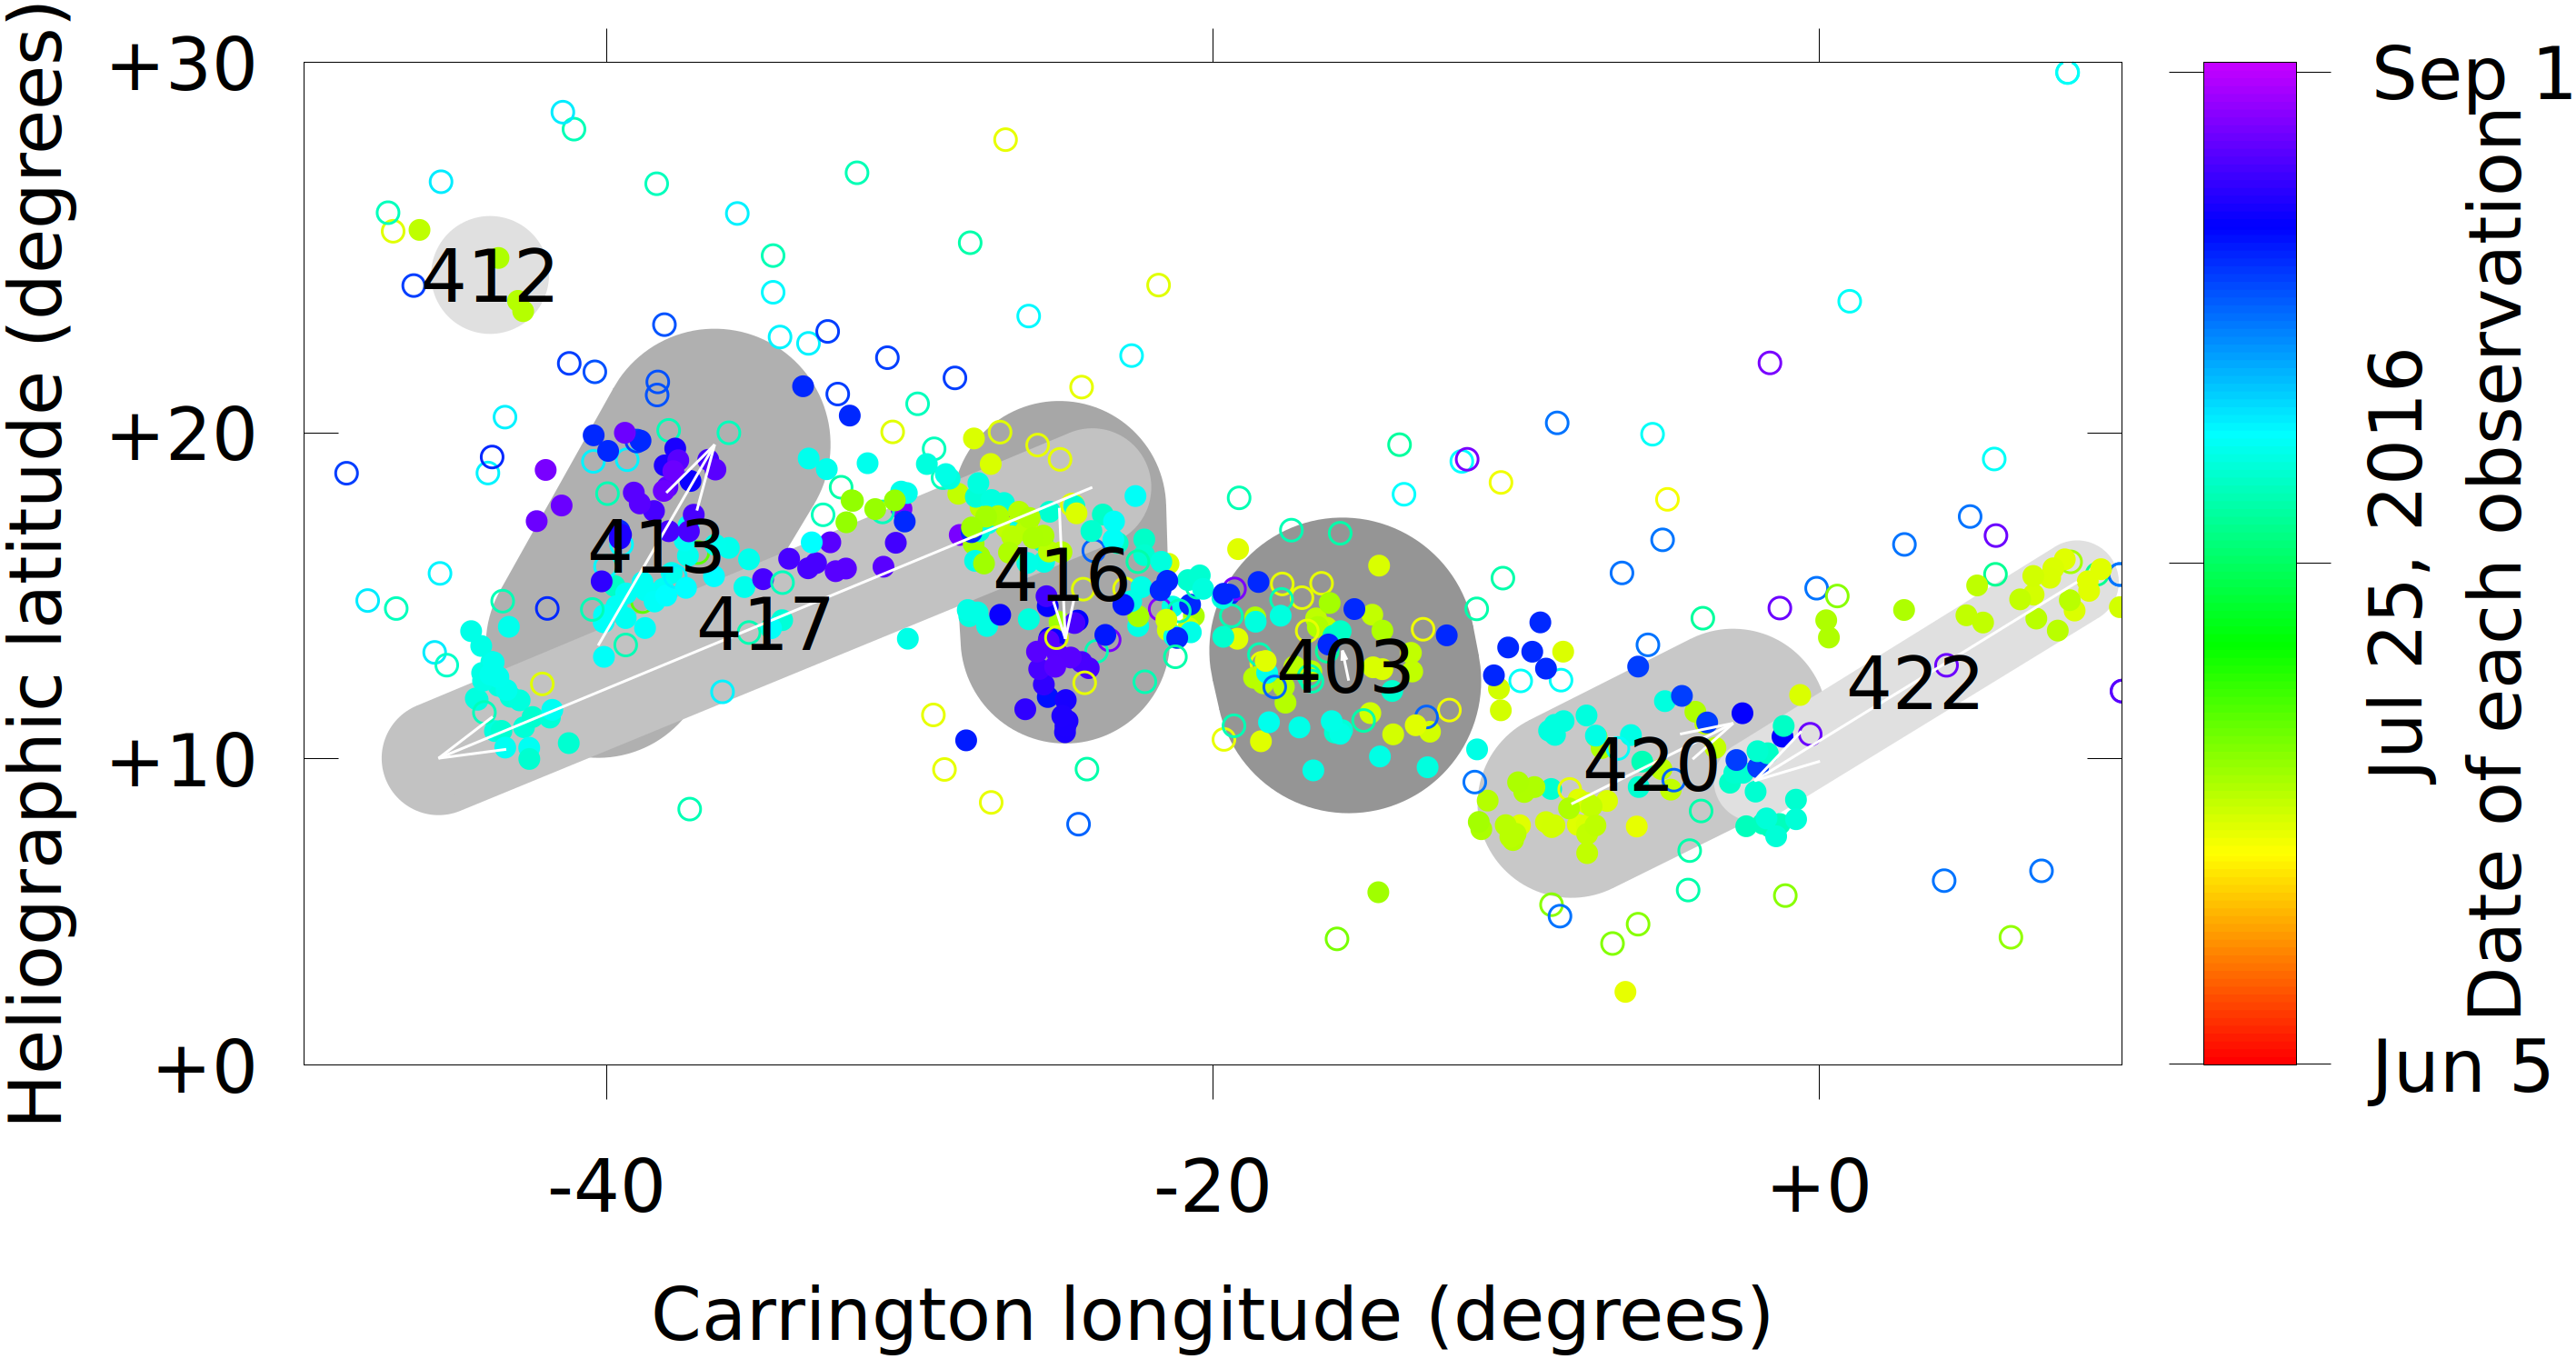
\includegraphics[width=8.8cm]{carrington3.png}
%\caption{Closeup of Figure \ref{carrington1} showing details of individual observation times with color.}
%\label{carrington3}
%\end{figure}
%
%\begin{figure} \centering 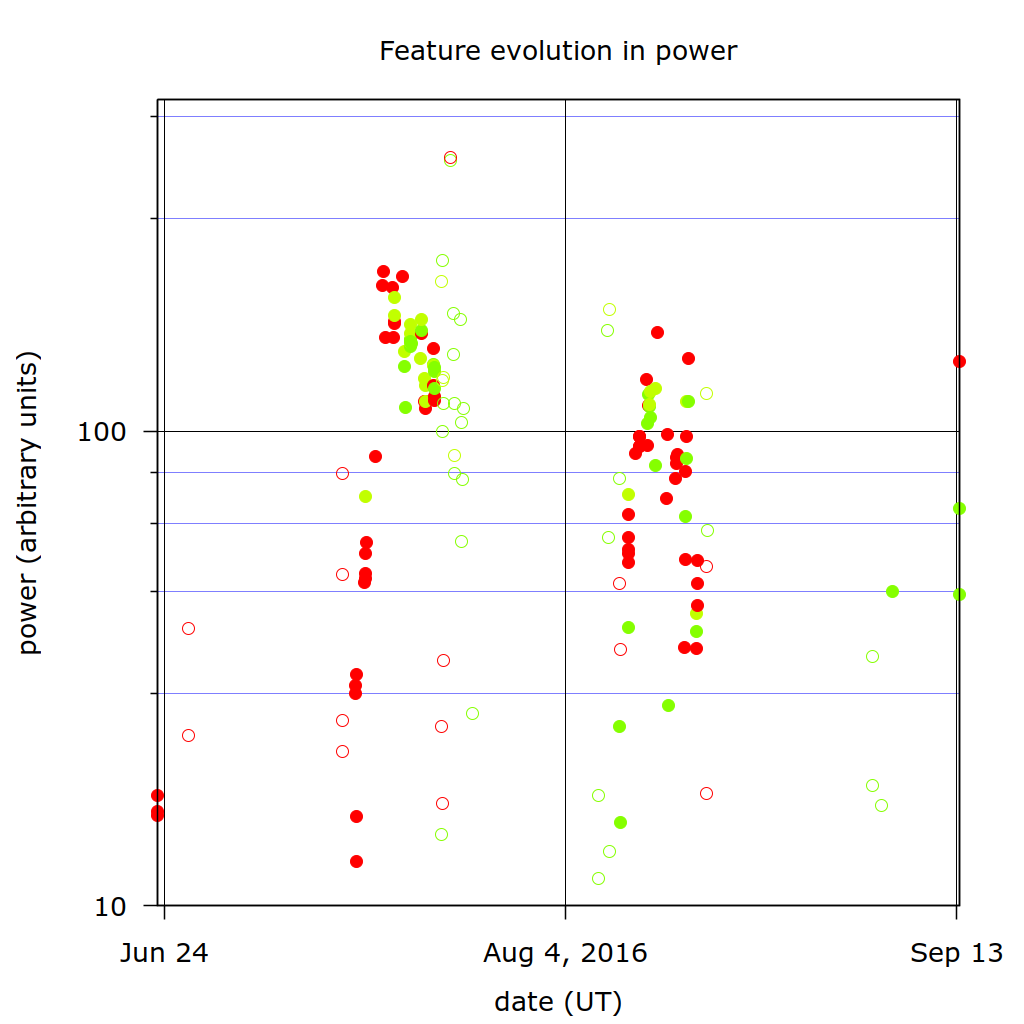
\includegraphics[width=8.8cm]{view_power_complex346.png}
%\caption{Radiative power of the active region 346 seen on top of the Quiet Sun Level. The units are nano steradians of Quiet Sun Level. Hollow points are observations which are more than $0.88$ disk radii from the center. The hollow points have greater uncertainty.}
%\label{complexpower} \end{figure}
%
%\begin{figure} \centering 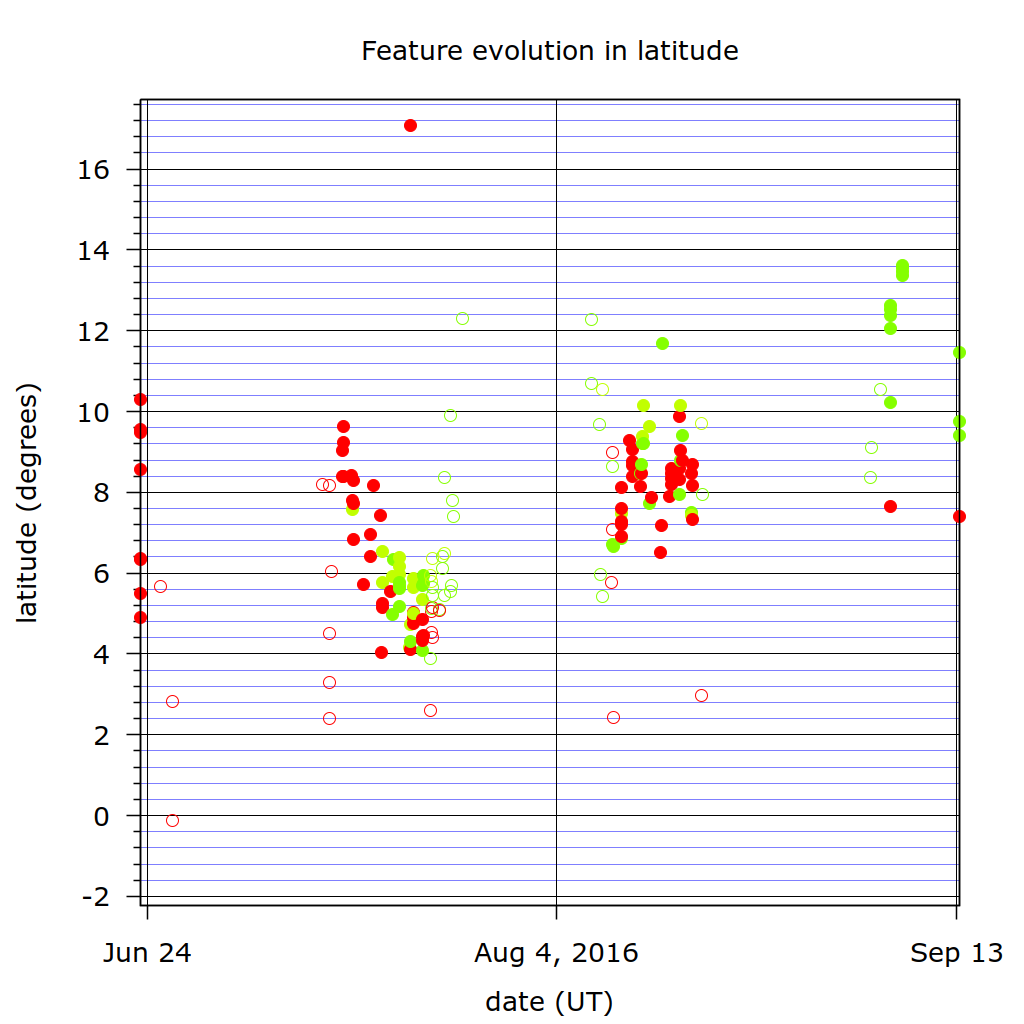
\includegraphics[width=8.8cm]{view_latitude_complex346.png}
%\caption{Latitude migration of the active region 346. Hollow points are observations which are more than $0.88$ disk radii from the center. The hollow points have greater uncertainty.}
%\label{complexlatitude} \end{figure}
%
%\begin{figure} \centering 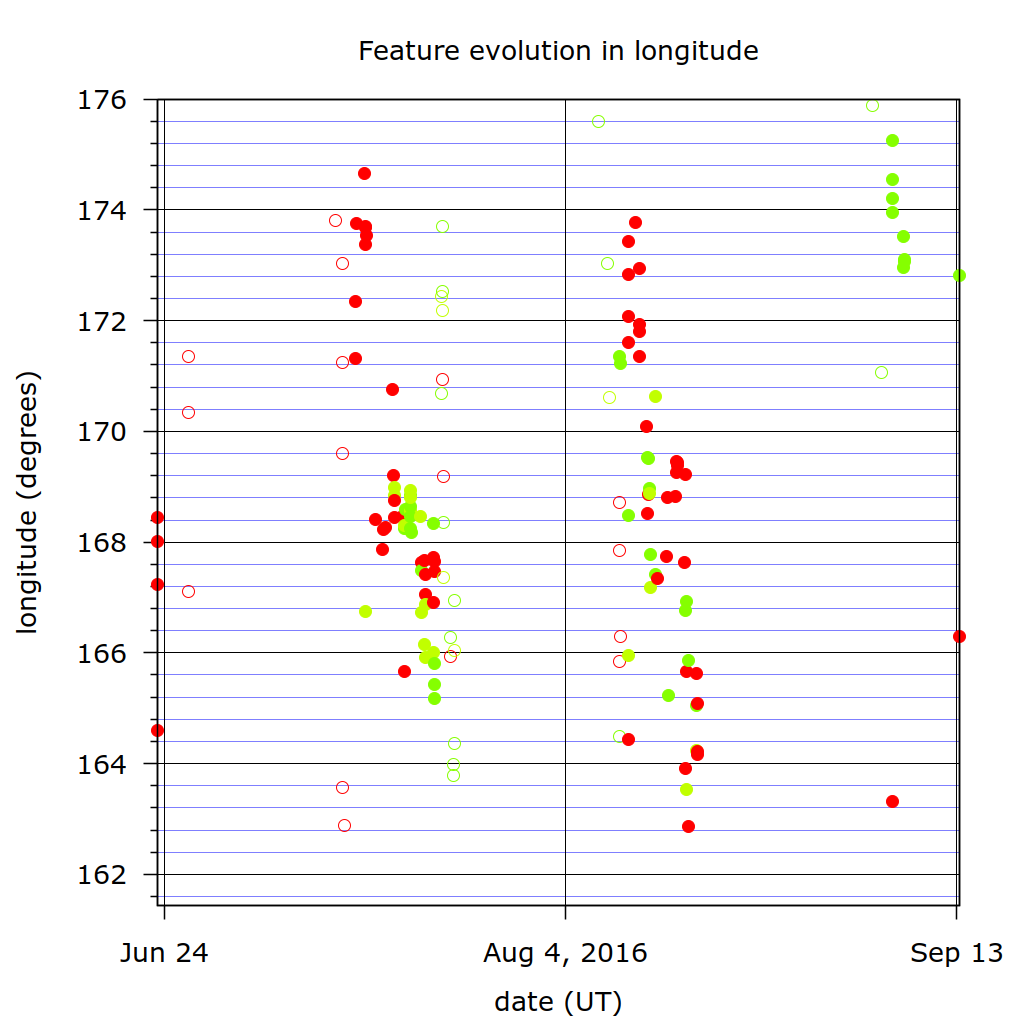
\includegraphics[width=8.8cm]{view_longitude_complex346.png}
%\caption{Longitude migration of the active region 346. Hollow points are observations which are more than $0.88$ disk radii from the center. The hollow points have greater uncertainty.}
%\label{complexlatitude} \end{figure}
%
%\begin{figure} \centering 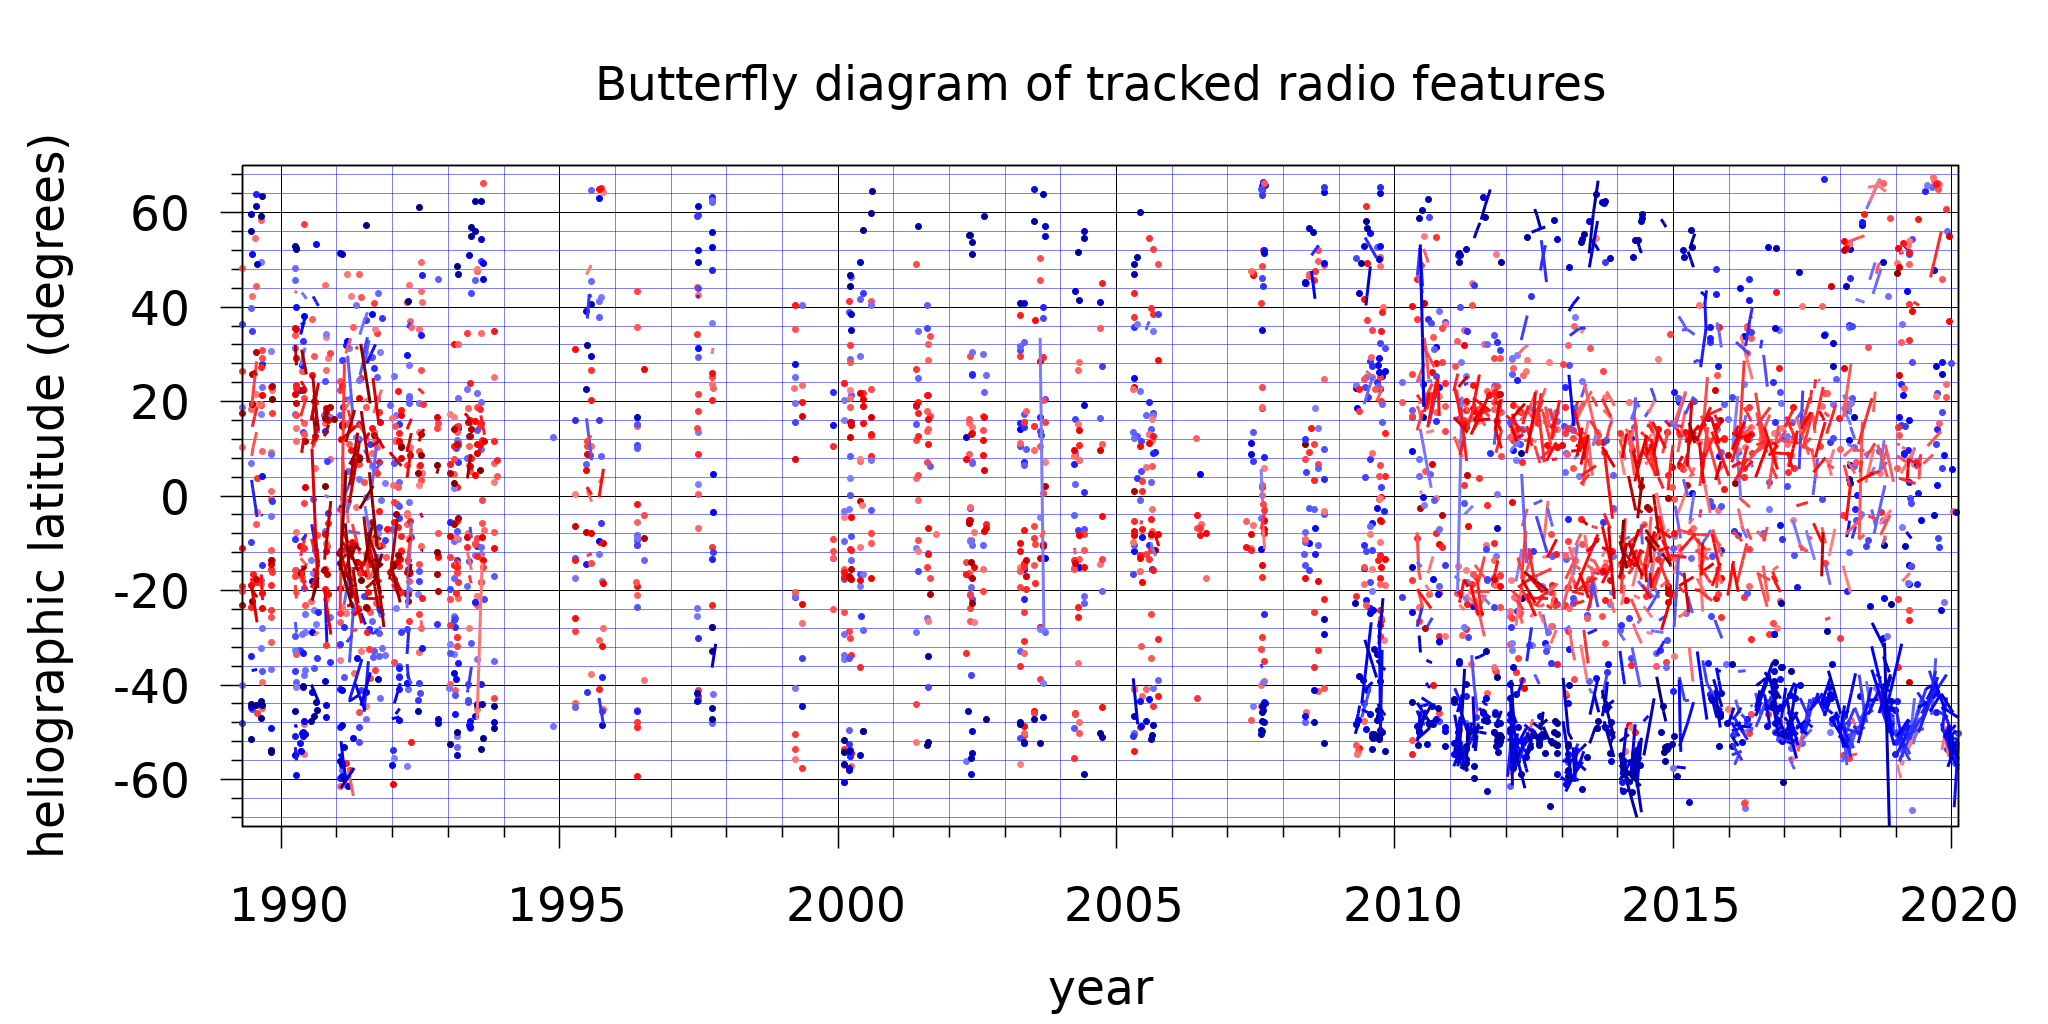
\includegraphics[width=8.8cm]{track_butterfly.png}
%\caption{Butterfly diagram drawn using tracked dim and bright features. When there is enough statistics, the track is shown as line which indicates its migration, otherwise only its average position is shown as a point. It is not yet clear why there is a mass of dim regions at the southern high latitudes, but in north, on cycle 24. The annual oscillation of the southern high latitude dim regions is probably due to observational effects, suggesting that the limb model needs to be upgraded. During the cycle 23, there are not observations every day, which results in scarser statistics and less migration information. As a result, most of the tracks are shown as points on cycle 23.}
%\label{track_butterfly} \end{figure}
%
%\begin{figure} \centering 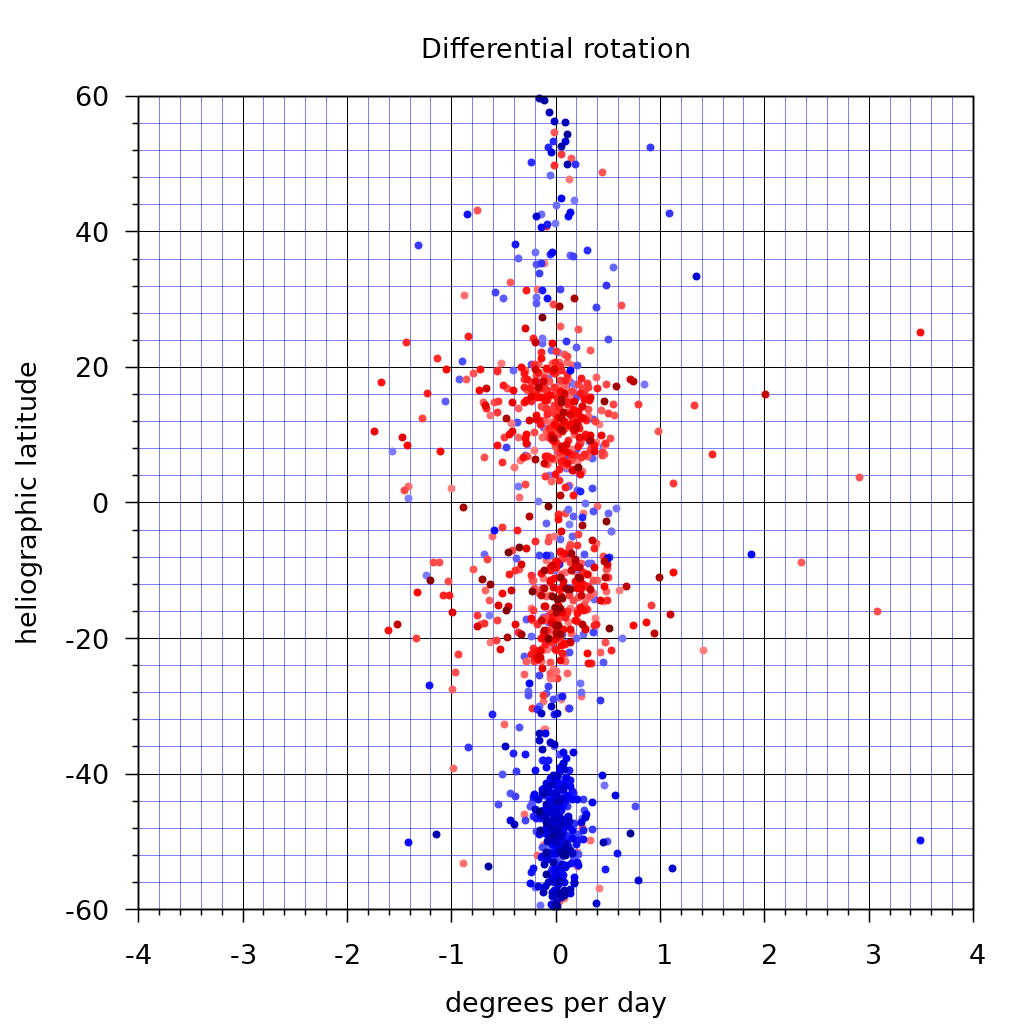
\includegraphics[width=8.8cm]{diffrot.png}
%\caption{Scatter plot of the bright and dim regions for which migration can be analyzed. At first glance, no significant differential rotation is observable.}
%\label{diffrot} \end{figure}
%
%\begin{figure} \centering 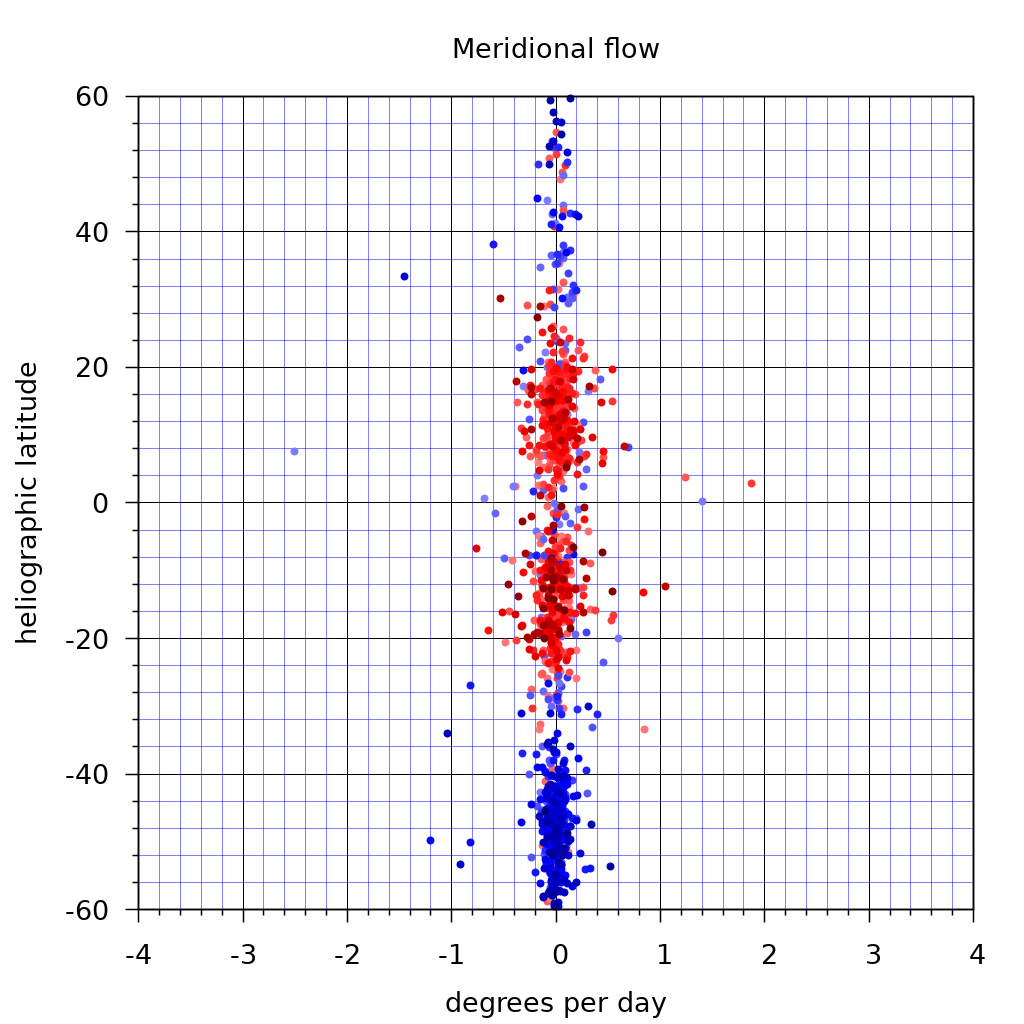
\includegraphics[width=8.8cm]{meridional.png}
%\caption{Scatter plot of the bright and dim regions for which migration can be analyzed. At first glance, no significant meridional flow is observable.}
%\label{meridional} \end{figure}
%
%\begin{figure} \centering 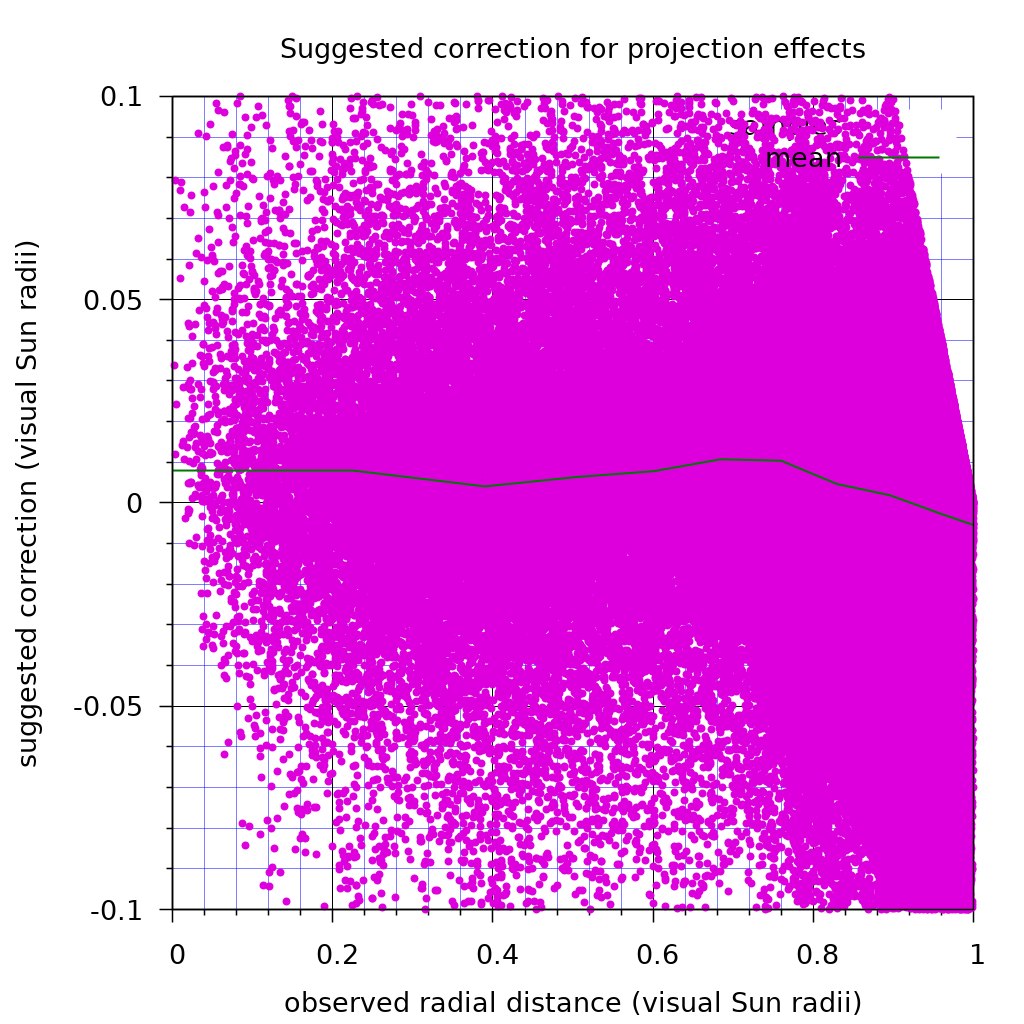
\includegraphics[width=8.8cm]{limb_offsets.png}
%\caption{Analysis of projection effects at the solar limb. As a tracked feature rotates along with the Sun, it is assumed to have a constant angular velocity on rotating heliographic surface, following a great circle. As its visual longitude changes, it is seen first near the east limb, then at the center, and finally at the west limb. We might expect convolution effects to bias its apparent position towards then visual center. This effect does not seem significant.}
%\label{limb_offsets} \end{figure}

\section{Discussion}\label{sect:discussion}

We have featured a software package for processing solar maps. The radio observations reproduce the butterfly diagram 
observed on sunspot data, and are able to see the extended cycle at high latitudes. We automatically detect bright and 
dim features from the maps and track them from map to map. This allows us to analyze their migration on heliographic 
surface. We also obtain various structural information from these regions.

\subsection{The big picture}

The radio samples in solar maps can be divided into three categories: \begin{itemize} \item Quiet Sun background \item 
Bright features \item Dim features. \end{itemize} Bright and dim features are a signal of activity. Our intention is to 
study the development and lifetime of this activity, for which we have developed algorithms for extracting these 
features from the maps. We also need to understand how the quiet Sun behaves, and for this purpose, any activity is 
excluded. The brightness of these quiet areas supposedly depend on heliographic latitude and the solar cycle. When these 
regions are observed, the ap:qparent brightness also depends on the distance from the visual center, due to atmospheric 
and antenna beam convolution effects. We want to measure these effects in order to properly compensate for them. We do 
not want any activity to affect these measurements, so we will benefit if we already know where the active and dim 
regions are. The compensation model consists of an implicit butterfly as well as a radial model for the brightness, and 
the expected brightness of a quiet region is taken as a product of these two.

Accurately understanding the radial effects in observations benefits the centering algorithm. Also, we benefit from 
prior knowledge of active regions since they can be excluded in the statistics which we feed into the centering 
algorithm. Otherwise the features at the limb would bias the center of the map.

Radial model also increases the dynamic radius of the map, and we are able to detect bright and dim features at the 
limb, although with increased noise. Each part of the model will benefit other parts and result in a data model of progressive accuracy, as outlined in Figure \ref{roadmap}.

Ultimately, all these three aspects, quiet, bright, and dim features, have a known physical origin, and their 
statistical appearance and characteristics can be reproduced in appropriate simulations.

%\begin{figure*} 
%\centering \scalebox{0.75}{\begin{tikzpicture}
%\node[textarea] (maps) {Mets\"ahovi solar intensity maps};
%\node[largeblock, right=5mm of maps] (calib) {\setlength\tabcolsep{0pt} \begin{tabular}{m{23mm}m{15mm}} Disk fitting and intensity calibration & 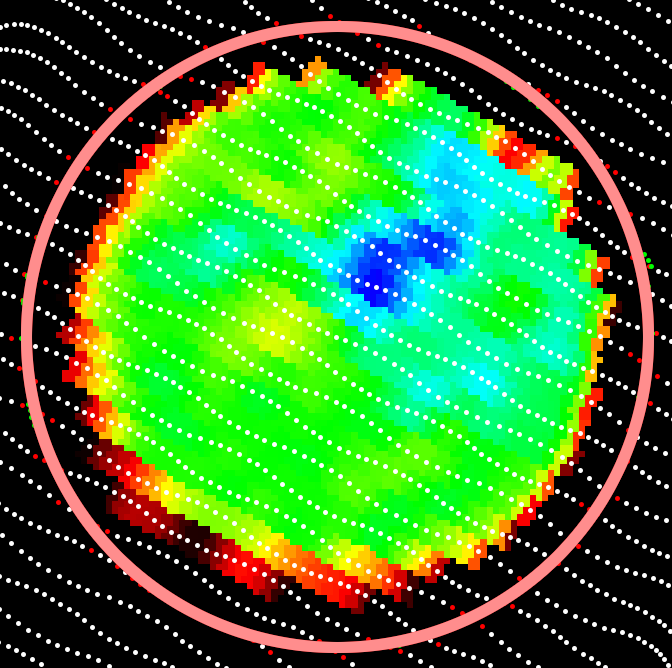
\includegraphics[width=15mm]{calib.png} \end{tabular}};
%\node[block, below right=15mm and -25mm of calib] (estimate) {Solar disk estimate from least squares approach};
%\node[largeblock2, above right=10mm and -50mm of calib] (dbase) {\setlength\tabcolsep{0pt} \begin{tabular}{m{23mm}m{25mm}} Bright and dim region database & 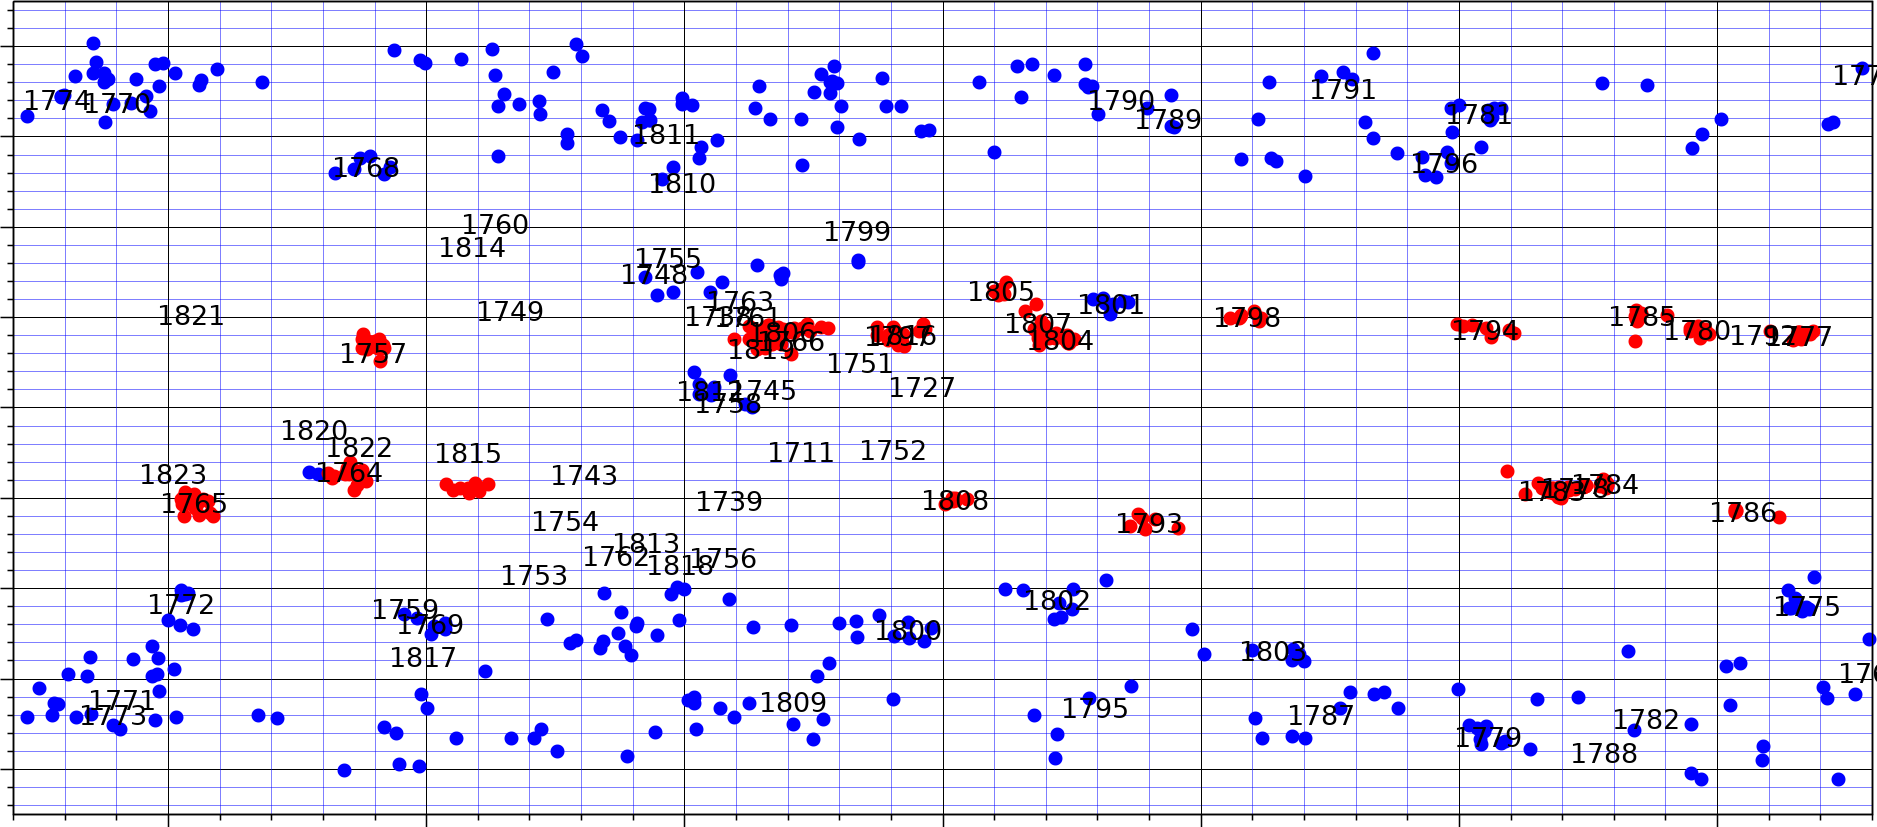
\includegraphics[width=25mm]{dbase.png} \end{tabular}};
%\node[largetextarea2, above right=-8mm and 5mm of estimate] (ibutterfly) {\setlength\tabcolsep{0pt} \begin{tabular}{m{23mm}m{25mm}} Implicit model for quiet sun butterfly & 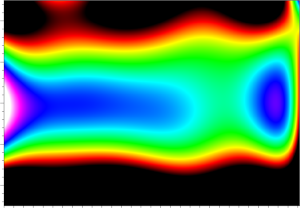
\includegraphics[width=25mm]{ibutterfly.png} \end{tabular}};
%\node[largetextarea2, below right=-8mm and 5mm of estimate] (lmodel) {\setlength\tabcolsep{0pt} \begin{tabular}{m{23mm}m{25mm}} Limb brightening and beam convolution model & 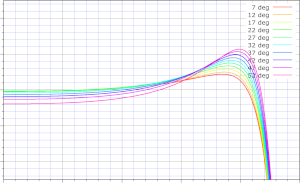
\includegraphics[width=25mm]{lmodel.png} \end{tabular}};
%\node[largetextarea, right=6mm of calib] (qbutterfly) {\setlength\tabcolsep{0pt} \begin{tabular}{m{23mm}m{25mm}} Quiet sun butterfly & 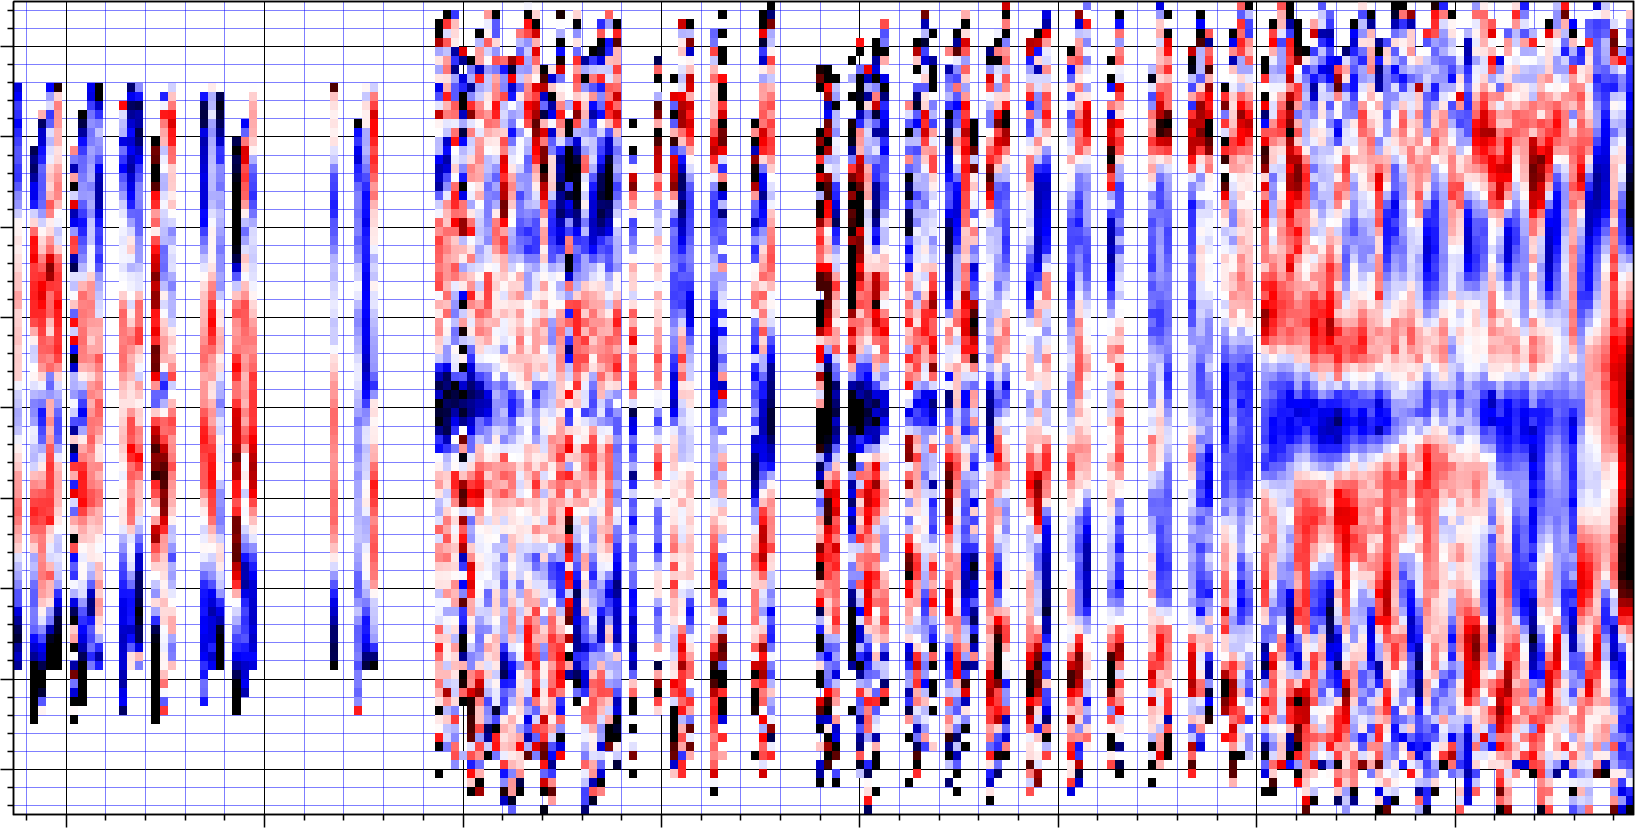
\includegraphics[width=25mm]{qbutterfly.png} \end{tabular}};
%\node[largetextarea, below right=-8mm and 5mm of dbase] (hbutterfly) {\setlength\tabcolsep{0pt} \begin{tabular}{m{23mm}m{25mm}} Bright region butterfly & 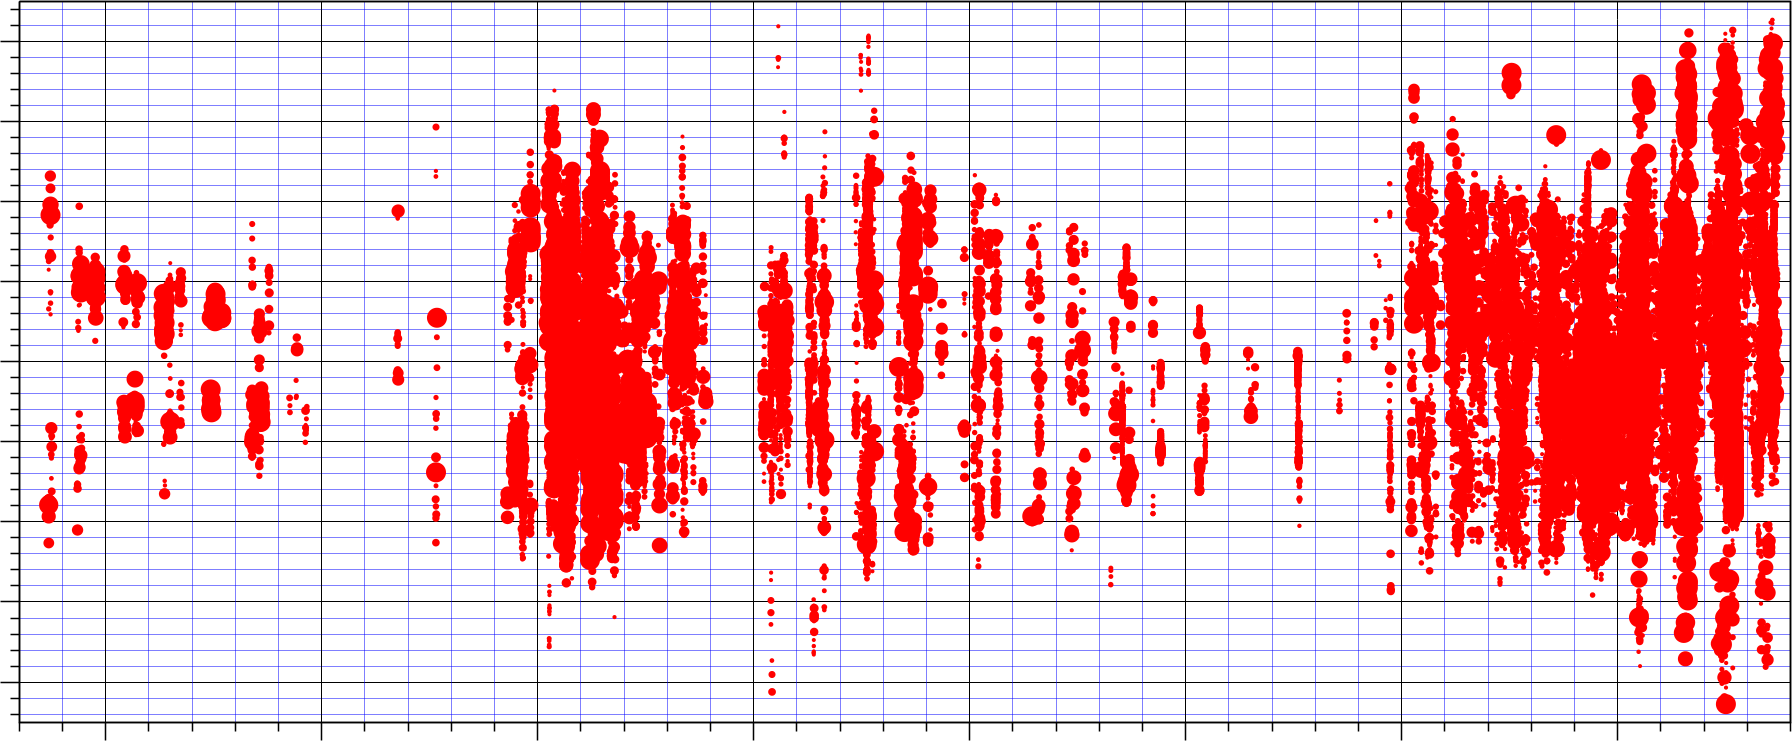
\includegraphics[width=25mm]{hbutterfly.png} \end{tabular}};
%\node[largetextarea, above right=-8mm and 5mm of dbase] (cbutterfly) {\setlength\tabcolsep{0pt} \begin{tabular}{m{23mm}m{25mm}} Dim region butterfly & 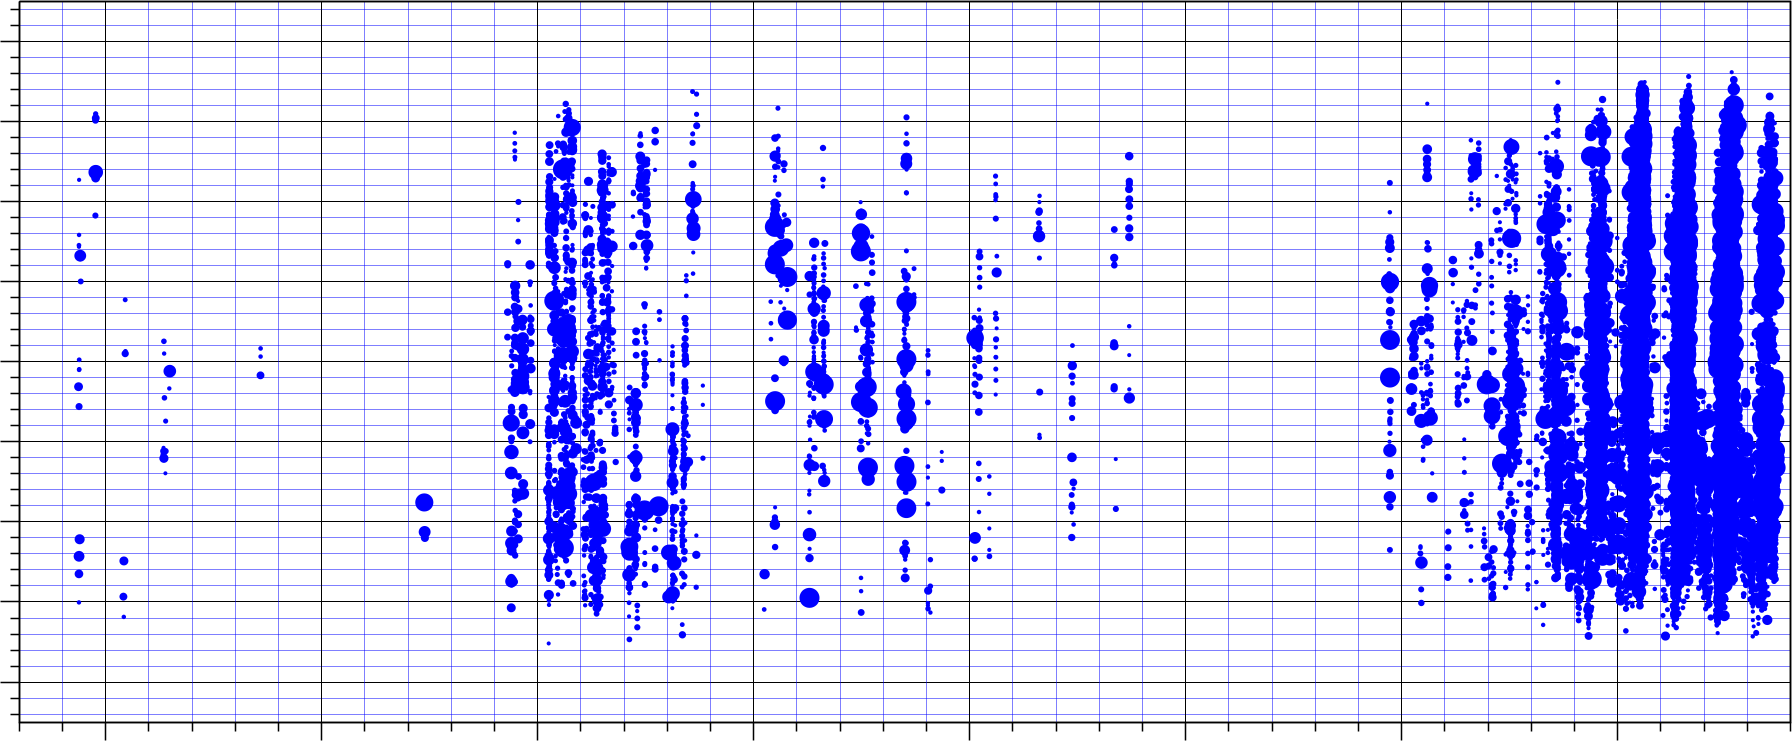
\includegraphics[width=25mm]{cbutterfly.png} \end{tabular}};
%\node[textarea2, right=10mm of hbutterfly] (compu) {Comparison with solar simulations};
%\node[dummy, left=4mm of calib.north] (calib_n1) {};
%\node[dummy, right=4mm of calib.north] (calib_n2) {};
%\node[dummy, left=4mm of calib.south] (calib_s1) {};
%\node[dummy, right=4mm of calib.south] (calib_s2) {};
%\node[dummy, left=4mm of dbase.south] (dbase_s1) {};
%\node[dummy, right=4mm of dbase.south] (dbase_s2) {};
%\node[dummy, left=4mm of estimate.north] (estimate_n1) {};
%\node[dummy, right=4mm of estimate.north] (estimate_n2) {};
%\draw[myarrow] (maps.east) -- (calib.west);
%\draw[myarrow] (calib_s1) -- (estimate_n1);
%\draw[myarrow] (estimate_n2) -- (calib_s2);
%\draw[myarrow] (calib_n1) -- (dbase_s1);
%\draw[myarrow] (dbase_s2) -- (calib_n2);
%\node[dummy, above=4mm of dbase.east] (dbase_e1) {};
%\node[dummy, below=4mm of dbase.east] (dbase_e2) {};
%\draw[myarrow] (dbase_e1) -- (cbutterfly.west);
%\draw[myarrow] (dbase_e2) -- (hbutterfly.west);
%\draw[myarrow] (calib.east) -- (qbutterfly.west);
%\node[dummy, above=6mm of estimate.east] (estimate_e1) {};
%\node[dummy, above=2mm of estimate.east] (estimate_e2) {};
%\node[dummy, below=2mm of estimate.east] (estimate_e3) {};
%\node[dummy, below=6mm of estimate.east] (estimate_e4) {};
%\node[dummy, above=2mm of ibutterfly.west] (ibutterfly_w1) {};
%\node[dummy, below=2mm of ibutterfly.west] (ibutterfly_w2) {};
%\node[dummy, above=2mm of lmodel.west] (lmodel_w1) {};
%\node[dummy, below=2mm of lmodel.west] (lmodel_w2) {};
%\draw[myarrow] (estimate_e1) -- (ibutterfly_w1);
%\draw[myarrow] (ibutterfly_w2) -- (estimate_e2);
%\draw[myarrow] (estimate_e3) -- (lmodel_w1);
%\draw[myarrow] (lmodel_w2) -- (estimate_e4);
%\node[dummy, above=4mm of compu.west] (compu_w1) {};
%\node[dummy, above=0mm of compu.west] (compu_w2) {};
%\node[dummy, below=4mm of compu.west] (compu_w3) {};
%\draw[myarrow] (cbutterfly.east) -- (compu_w1);
%\draw[myarrow] (hbutterfly.east) -- (compu_w2);
%\draw[myarrow] (qbutterfly.east) -- (compu_w3);
%\end{tikzpicture}} \caption{Roadmap for extracting valuable information from the solar maps.} \label{roadmap} \end{figure*}
%

\begin{acknowledgements}
\end{acknowledgements}

% WARNING
%-------------------------------------------------------------------
% Please note that we have included the references to the file aa.dem in
% order to compile it, but we ask you to:
%
% - use BibTeX with the regular commands:
%   \bibliographystyle{aa} % style aa.bst
%   \bibliography{Yourfile} % your references Yourfile.bib
%
% - join the .bib files when you upload your source files
%-------------------------------------------------------------------

\bibliographystyle{aa}
\bibliography{main_P1}

\end{document}

